
% this file is called up by thesis.tex
% content in this file will be fed into the main document

%: ----------------------- introduction file header -----------------------
%\begin{savequote}[50mm]
%The logic of validation allows us to move between the two limits of dogmatism and skepticism.
%\qauthor{Paul Ricoeur}
%\end{savequote}


\chapter{El teorema de Nielsen}
\label{cha:El teorema de Nielsen}

% the code below specifies where the figures are stored
%\ifpdf
%    \graphicspath{{4_experiments_and_results/figures/PNG/}{4_experiments_and_results/figures/PDF/}{4_experiments_and_results/figures/}}
%\else
%    \graphicspath{{4_experiments_and_results/figures/EPS/}{4_experiments_and_results/figures/}}
%\fi


%-------------------------------------------------------------------------

%\cite{turing1950computing}

En este cap\'itulo proponemos un teorema sobre la acci\'on discontinua de  grupos de transformaciones que pretendemos aplicar al caso del grupo de monodrom\'ia de la ecuaci\'on hipergeom\'etrica.

Todo en  este cap\'itulo es pensado en el sentido de Poincar\'e y hacemos un breve recordatorio de los conceptos que ocupamos durante el mismo.

Tratamos de dar una caracterizaci\'on de los grupos propiamente discontinuos de transformaciones lineales fraccionales con c\'irculo principal en el sentido de la teor\'ia de automorfismos.
Representamos al plano hiperb\'olico como una regi\'on circular en el plano complejo, este modelo llamado el disco de poincar\'e se divide en dos partes de $\lbrace z | |z| \leq 1 \rbrace$,el interior
le denominamos $D =\lbrace z | |z| <1 \rbrace$ y la frontera la denominamos  $E =\lbrace z| |z| =1  \rbrace$.  Todas las cosecuencias geom\'etricas las entendemos en el sentido no-euclidio. Tambi\'en denotamos por $\mathbb{H} ^{+}$ al modelo hiperb\'olico del semiplano.\\



Llamamos puntos finales a los extremos de una recta situados en
el c\'irculo infinito, e identificamos tres tipos de relaciones entre las rectas, a saber;
concurrentes, paralelas y divergentes. \\

\begin{defn}
Las rectas Paralelas son dos rectas que tienen un punto
final en com\'un.\\
Las rectas Concurrentes son las que se intersectan en $D$.
\\
Las rectas Divergentes son las que no se intersectan en
nig\'un lugar. \\
\end{defn}



\begin{figure}[h]
  \centering
  % Requires \usepackage{graphicx}
  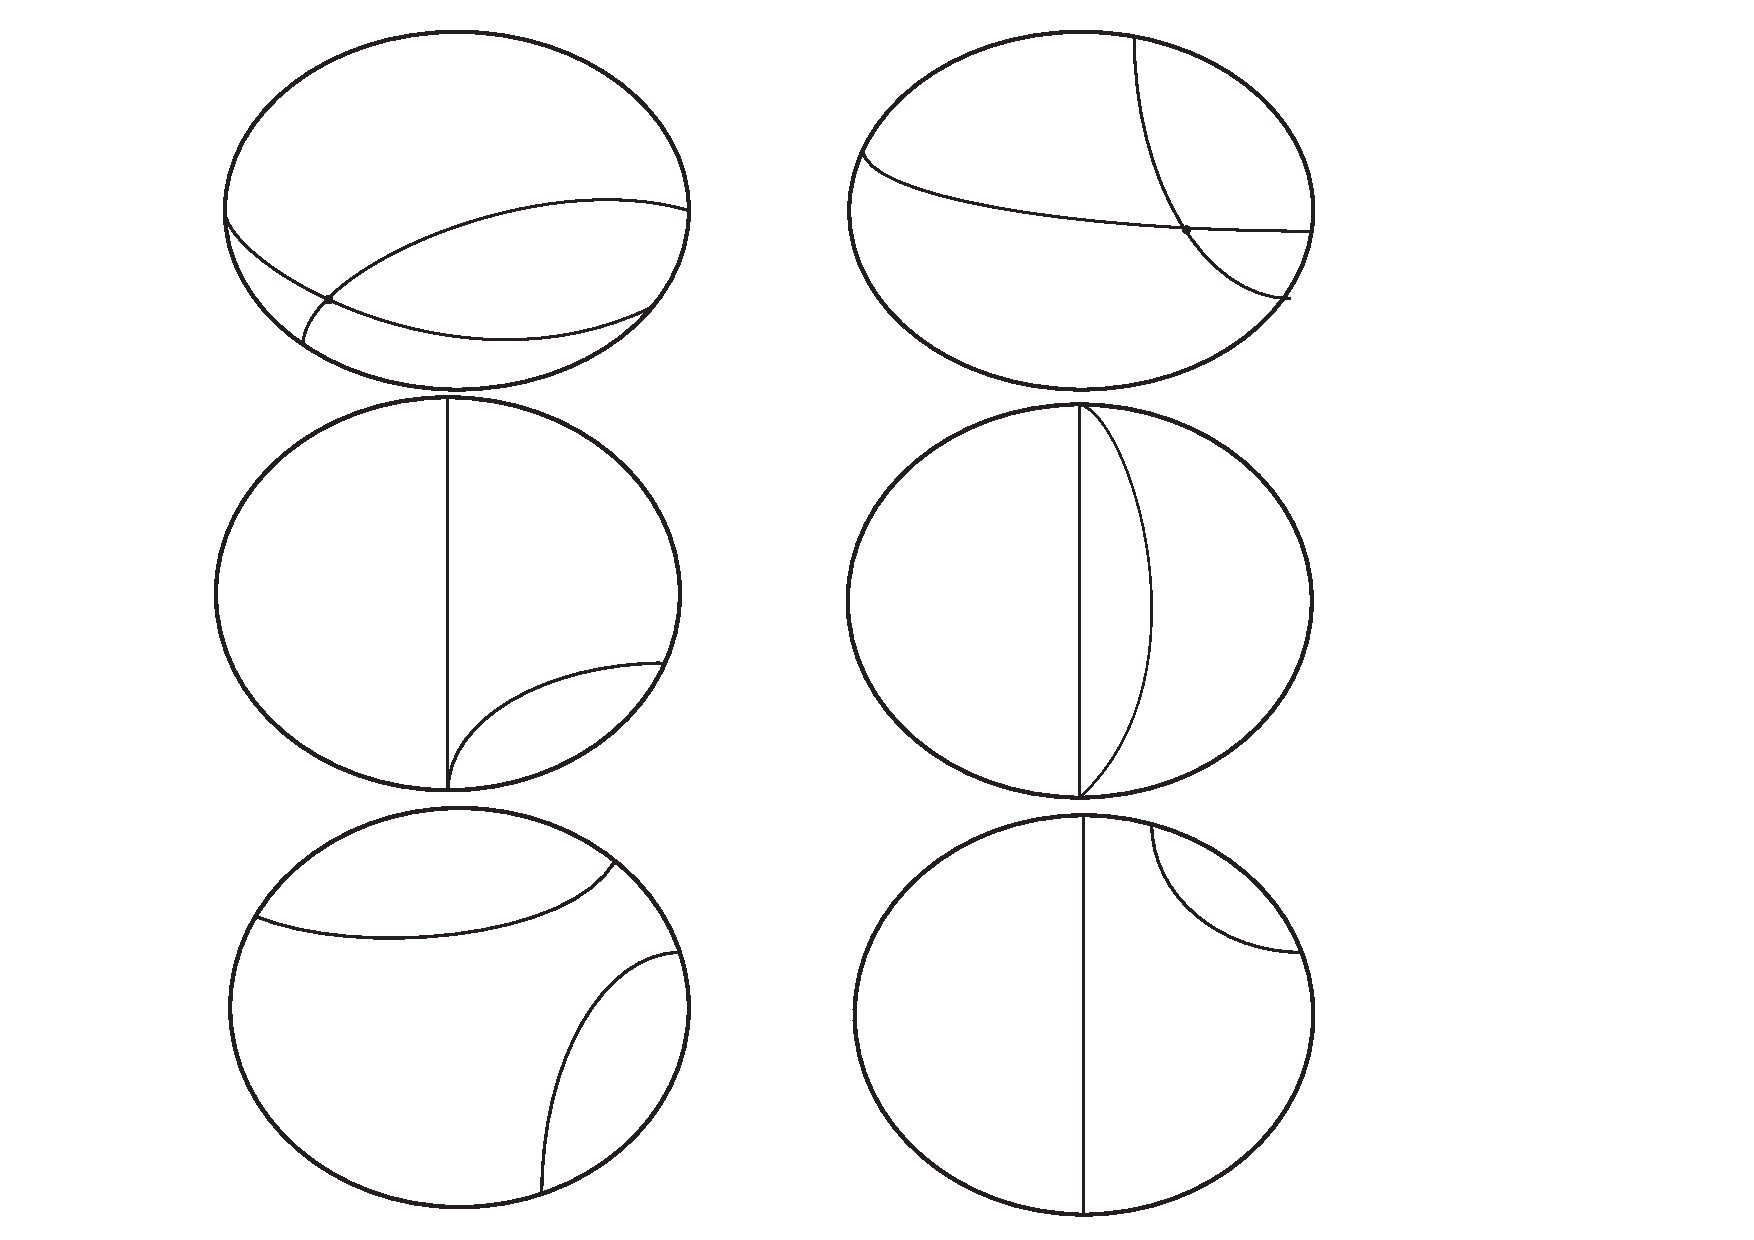
\includegraphics[width=10cm]{rectas-concurrentes-paralelas-divergentes.pdf}\\
  \caption{Rectas hiperb\'olicas concurrentes, paralelas y divergentes respectivamente.}%\label{}
\end{figure}


Los \textbf{Horociclos} son c\'irculos tangentes a alg\'un punto en la
frontera $E$ de $S^{1}$.Es importante dejar en claro que los Horociclos no son geod\'esicas. \\


Los \textbf{hiperciclos} se forman por una recta $\emph{L}$ y un
punto $\textbf{P}$ fuera de ella, el hiperciclo es  el lugar geom\'etrico
de todos los puntos a distancia $d_{H}(\textbf{P},\emph{L})$,  de
$\emph{L}$ y del mismo lado de $P$.  $d_{H}$ es la distancia hiperb\'olica.
 De igual manera los hiperciclos no son geod\'esicas. \\


Dividiremos las transformaciones isom\'etricas en dos grupos, las
que preservan la orientaci\'on y las que no. En el grupo de las que
preservan la orientaci\'ion distinguimos tres tipos distintos de
transformaciones; \\

\begin{defn}
Las transformaciones \textbf{parab\'olicas} tienen un punto fijo en
$E$ y dado un horociclo $K$ tangente en dicho punto fijo a $E$, esta
transformaci\'on tiene un desplazamiento fijo en $K$.


Las tranformaciones \textbf{el\'ipticas} tienen un punto fijo en $D$
y un \'angulo fijo $\phi$ de rotaci\'on en torno al punto fijo.


Las transformaciones \textbf{hiperb\'olicas} tienen dos puntos fijos
en $E$ y una recta invariante, la recta que pasa por dichos puntos
fijos la llamamos eje de la transformaci\'on.


\begin{figure}[h]
  \centering
  % Requires \usepackage{graphicx}
  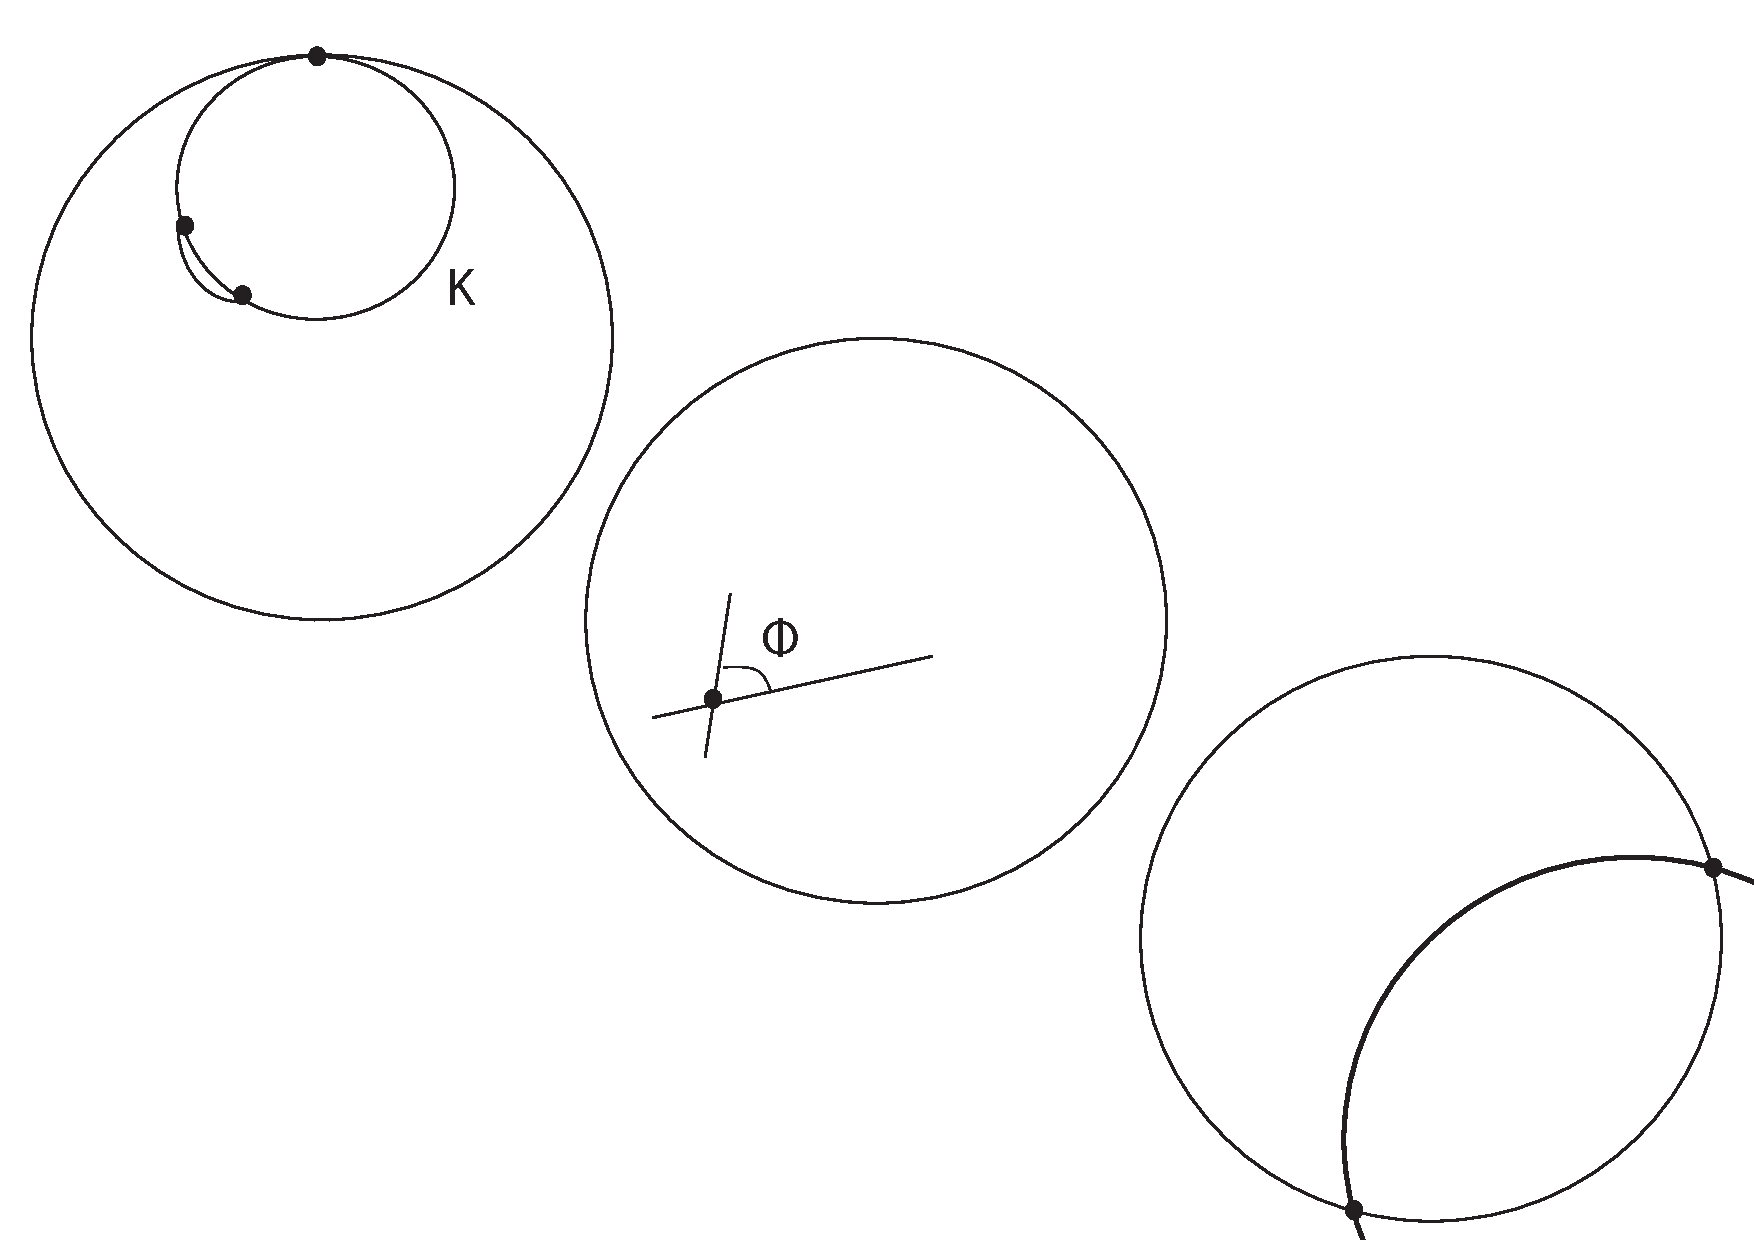
\includegraphics[width=8cm]{definicion40.pdf}\\
  \caption{Representaci\'on de los puntos importantes en las transformaciones hperb\'olicas}\label{definicion40}
\end{figure}


\end{defn}

Si $G$ es un grupo de transformaciones isom\'etricas, un punto
invariante para $G$ es un punto fijo bajo todos los elementos de $G$, de
una manera similar pensamos en una recta invariante. \\

Un par de conjuntos de puntos $M$ y $M'$ en $D + E$ son equivalentes respecto a
$G$ si existe $f \in G$ tal que $M = fM'$. El total de conjuntos
equivalentes de $M$ se denota como la familia $GM$ llamada clase de
equivalencia de $M$, en esta familia si $f_{1},f_{2} \in G  $ y
$f_{1} \neq f_{2 }$ entonces $f_{1}M \neq f_{2}M$ sin importar que
como conjunto sean iguales. \\

\begin{defn}
Decimos que $G$ es discontinuo en un punto $x \in D$,si $x$ no es un
punto de acumulaci\'on de la clase $Gx$, si esto sucede $Gx$ no
tiene puntos de acumulaci\'on en $D$
\end{defn}

\begin{prop}
Si $G$ es discontinuo en $x$, $G$ no tiene puntos de acumulaci\'on en $D$.
\end{prop}

\textit{Prueba}:

Supongamos que $G$ es discontinuo en $x$, existe $m$ tal que $\forall \ i,j, \  d_{H}(g_{i}x,g_{j}x) > m$, de otro modo $x$ ser\'ia un punto de acumulaci\'on de $Gx$. Sea $y$ un punto arbitrario de $D$ y sea $U_{r}$ una vecindad de $y$ de radio $r < m$, entonces a lo m\'as hay un punto $gx$ de $Gx$ en $U_{r}$, si tomamos $V_{r'}$ vecindad de $y$ con $r' < d_{H}(gx,y)$, esa vecindad no contiene puntos de $Gx$. $_{\square}$

Esto implica que si $G$  es discontinuo en un punto de  $D$ entonces es discontinuo en todo
$D$.\\

Las \'unicas isometr\'ias de $\mathbb{H}^{+} $ que preservan la orientaci\'on
son las de $PSL(2,\mathbb{R})$, las transformaciones mencionadas con
anterioridad se encuentran en este grupo. Si $f \in PSL(2,\mathbb{R})$ y $g$  otra transformaci\'on  entonces $gfg^{-1}$ es de la misma clase que $f$.\\

Llamaremos \textbf{reversiones} a las transformaciones que invierten
la orientaci\'on, las reversiones son las \textbf{reflexiones}
respecto a una recta, y las reflexiones compuestas con elementos
hiperb\'olicos a las que llamamos \textbf{h-reflexiones}. \\


La reflexi\'on respecto a una recta hiperb\'olica es la reflexi\'on
respecto a una circunferencia euclidiana. \\


\begin{thm} \label{Teorema-nielsen} [Teorema de Nielsen]
Una condici\'on necesaria y suficiente para que un grupo de
transformaciones isom\'etricas en el plano hiperb\'olico sin puntos
ni lineas invariantes sea discontinuo en $D $ es que los puntos
fijos de los elementos el\'ipticos del grupo, si los hay, no se
acumulen en $D$

\end{thm}

La condici\'on de que no tenga puntos ni rectas invariantes es
necesaria, como podemos ver en los siguientes casos.

\begin{enumerate}
\item Si $G$ es un grupo de elementos parab\'olicos con un mismo punto
fijo al infinito.
\item Si $G$ es un grupo de elementos hiperb\'olicos con una recta fija
dada.
\end{enumerate}

Ninguno de los anteriores contiene elementos el\'ipticos sin embargo
ninguno es discontinuo en $D$.\\

Si $G$ contiene reversiones  y $H$ es un subgrupo de $G$ y adem\'as $H
\subseteq PSL(2,\mathbb{R})$ se tiene que $H$  es normal y de \'indice 2. Es normal ya que si $f \in H$
para cualquier elemento $g \in G$ se tiene que $gfg^{-1}$ es del
mismo tipo que $f$ por lo que $gfg^{1} \in H$, es de \'indice 2,
para ver esto basta probar que si $f,g \in G - H$ entonces $f \cong
g$ equivalentemente que $fg^{-1} \in H$, dado que $f , g$ revierten
orientaci\'on  se tiene que $fg^{-1}$ conserva la orientaci\'on y
por lo tanto esta en
$H$. \\

Una clase de equivalencia $Gx$ es la suma de las clases $Hx$ y $Hgx$
con $g$ una reversi\'on en $G$ ($H \cup Hg = G \Rightarrow Hx \cup
Hgx = Gx $ ), por lo que se concluye que $G$ y $H$
son ambos discontinuos en $D$ o ambos no lo son. En otras palabras $H$ es discontinuo en $D$ si y solo si $G$ lo es.


\begin{prop} Si $G$ no tiene rectas ni puntos invariantes tampoco los
tiene $H$.
\end{prop}

\textit{Prueba}:

 Supongamos que $H$ deja invariantes un punto en $D +E$,
pero ning\'un otro punto (y por tanto ninguna recta), como $G$ no
deja puntos invariantes, existe $g \in G $ tal que $gc \neq c$ luego
el subgrupo $gHg^{-1}$ deja invariante $gc$ pero ningun otro punto en
$D+E$ pero como $H \vartriangleleft G$ se tiene que  $gHg^{-1}=H$ y
como $gc \neq c $ implica que $H$ fija $c$ y $gc$ lo cual es una
contradicci\'on, concluimos que $H$ no deja puntos invariantes. Un
razonamiento an\'alogo nos enseña que $H$ no deja rectas invariantes. $_{\square}$ \\


Desde ahora  $G$ denotar\'a un subgrupo de $PSL(2,\mathbb{R})$ sin
puntos ni rectas invariantes. \\

Ahora probamos el \textbf{Teorema} \ref{Teorema-nielsen} para el caso cuando el grupo tiene elementos el\'ipticos.

\textit{Prueba}:

Primero probaremos que si los puntos fijos de los elementos el\'ipticos se
acumulan $\Rightarrow$ $G$ no es discontinuo en $D$ \\

Supongamos que los puntos fijos de los elementos el\'ipticos se
acumulan en $D$ (tiene un punto de acumulaci\'on en $D$), es posible
encontrar una sucesi\'on de puntos fijos que convergen al punto de
acumulaci\'on digamos $x$ (por ser espacio m\'etrico) y sean estos $y_{1},y_{2},...$ y
$f_{1},f_{2},...$ los respectivos elementos el\'ipticos. Por un lado
$d_{H}(y_{i},x) \leq \epsilon $ para $i$ adecuada, considerando $\lbrace
f_{i}x\rbrace$ podemos notar que

$$ d_{H}(f_{i}x,x) \leq d_{H}(f_{i}x,y_{i}) + d_{H}(y_{i},x) = 2d_{H}(y_{i},x)$$

Lo anterior debido a que $f_{i}$ fija $y_{i}$ y que es una
isometr\'ia. Luego entonces $f_{i}x \rightarrow x$, es decir $Gx$ se
acumula en $x$  por tanto $G$ no es discontinuo en $x$ y por lo
tanto no lo es en $D$.\\

Si los puntos fijos de los elementos el\'ipticos no se acumulan en $D$
$\Rightarrow$ $G$ es discontinuo en $D$.\\

Sea $c$ un punto fijo de alg\'un elemento el\'iptico en $G$. Basta notar que $Gc$ contiene solo puntos fijos de elementos el\'ipticos de $G$, observando que para $g(c) \in Gc$ el elemento $gfg^{-1} \in G$ lo deja fijo si $f $ es un elemento el\'iptico que fija $c$, luego $c$ no es un punto de acumulaci\'on de $Gc$ ya que los puntos fijos de elementos el\'ipticos no se acumulan, entonces $G$ es discontinuo en $c$ y por lo tanto $G$ es disontinuo en $D$.

%Elegimos un elemento el\'iptico $f $ y sea $c$ su punto fijo, como
%$G$ no tiene puntos invariantes existe $g \in G $ tal que $g(c) \neq
%c$ y adem\'as $g(c)$ es punto fijo de $gfg^{-1} $ que es de igual
%manera un elemento el\'iptico. Sea $G(c)$ el subgrupo de $G$ de
%elementos el\'ipticos con punto fijo $c$ entonces la cardinalidad $\sharp G(c) <
%\infty$, para ver esto notemos 2 cosas;

%\begin{enumerate}
%\item $hg(c)$ es punto fijo de alg\'un elemento el\'iptico en $G$ a
%saber $hgfg^{-1}h^{-1}, \forall h \in G(c)$
%\item $d_{H}(g(c),c)=d_{H}(hg(c),h(c))=d_{H}(hg(c),c)$
%\end{enumerate}

%Esto implica que el conjunto $G(c)g(c)$ esta contenido en una
%circunferencia con centro $c$, si $G(c)g(c)$ es infinito y dado que la
%circunferencia es compacta $G(c)g(c)$ tendria un punto de
%acumulaci\'on en dicha circunferencia lo cual contradice nuestra
%hip\'otesis, entonces necesariamente  $\sharp G(c) < \infty$, luego
%se tiene que $Gc$ se compone de puntos fijos de elementos
%el\'ipticos (gc es punto fijo de $gfg^{-1}$ ) en $G$. \\

%Si $gc \in Gc$ se tiene  $\sharp G(c) = \sharp G(gc)$ ya que se
%tiene la biyecci\'on $f \mapsto gfg^{-1}$ con inversa $h \mapsto g^{-1}hg$.



\section{El lema de los elementos hiperb\'olicos con ejes divergentes}

\begin{lem} \label{lema1}
Sean f y g elementos hiperb\'olicos cuyos ejes son divergentes y
cuyos desplazamientos $\lambda$ miden lo mismo pero tienen sentidos
opuestos, y sea $\delta$ la distancia entre sus ejes, entonces $fg$
es el\'iptico, parab\'olico o hiperb\'olico dependiendo de
$$senh \frac{1}{2} \delta senh \frac{1}{2} \lambda    \left \{ \begin{matrix} > 1 & \mbox{ }\mbox{ }
\\ =1 & \mbox{ }\mbox{ } \\ <1 \mbox{} {}\end{matrix}\right. $$
\end{lem}

\textit{Prueba}:

Como los ejes son divergentes existe una normal com\'un a ambos y a
esta recta le llamamos $s'$, denotemos a los ejes de $f$ y $g$ como
$A_{f}$ y $A_{g}$ respectivamente, entonces la normal que
mencionamos antes corta a $A_{f}$ en $a$ y a $A_{g}$ en $a'$ (Fig. \ref{lemma1-dem1}) y
elegimos $b,b'$ en $A_{f}$ y $A_{g}$ respectivamente  de tal manera
que $d_{H}(a,b)=d_{H}(a',b')= \frac{1}{2} \lambda$ y adem\'as en la
direcci\'on que se desplaza $f$. Sean $s,s''$ las rectas normales a
$A_{f},A_{g}$ en $b, b'$ y por abuso de notaci\'on las reflexiones
respecto a estas rectas y $s'$ se denotaran de la misma manera. (Fig. \ref{lemma1-dibujo4}) \\ \\

Queremos ver que tenemos la relaci\'on $f=ss'$, es claro que $ss'$
preserva $A_{f}$ ya que $s'$ lo preserva y $s$ tambi\'en por ser
normal a este eje (las circunferencias ortogonales son invariantes bajo inversiones
entre  ellas), para ver que tiene el mismo sentido que $f$
basta ver hacia donde desplaza un punto y es f\'acil si tomamos $a$ que
queda fijo bajo $s'$ y bajo $s$ se desplaza en la misma direcci\'on
que $f$, por \'ultimo hay que verificar que $d_{H}(x,ss'x) = \lambda
$ pero como $ss'$ preserva la orientaci\'on y tiene dos puntos fijos
(los puntos finales del eje fijo) necesariamente tiene que ser un
elemento hiperb\'olico y para saber cuanto mide su desplazamiento de
nuevo basta verificarlo para un punto en la recta fija y tomando 
de nuevo $a$ notamos que $d_{H}(a,ss'a)= d_{H}(a,sa)= \lambda$, en
conclusi\'on $f=ss'$ y un proceso an\'alogo nos permite probar que
$g=s's''$. \\

\begin{figure}[h]
  \centering
  % Requires \usepackage{graphicx}
  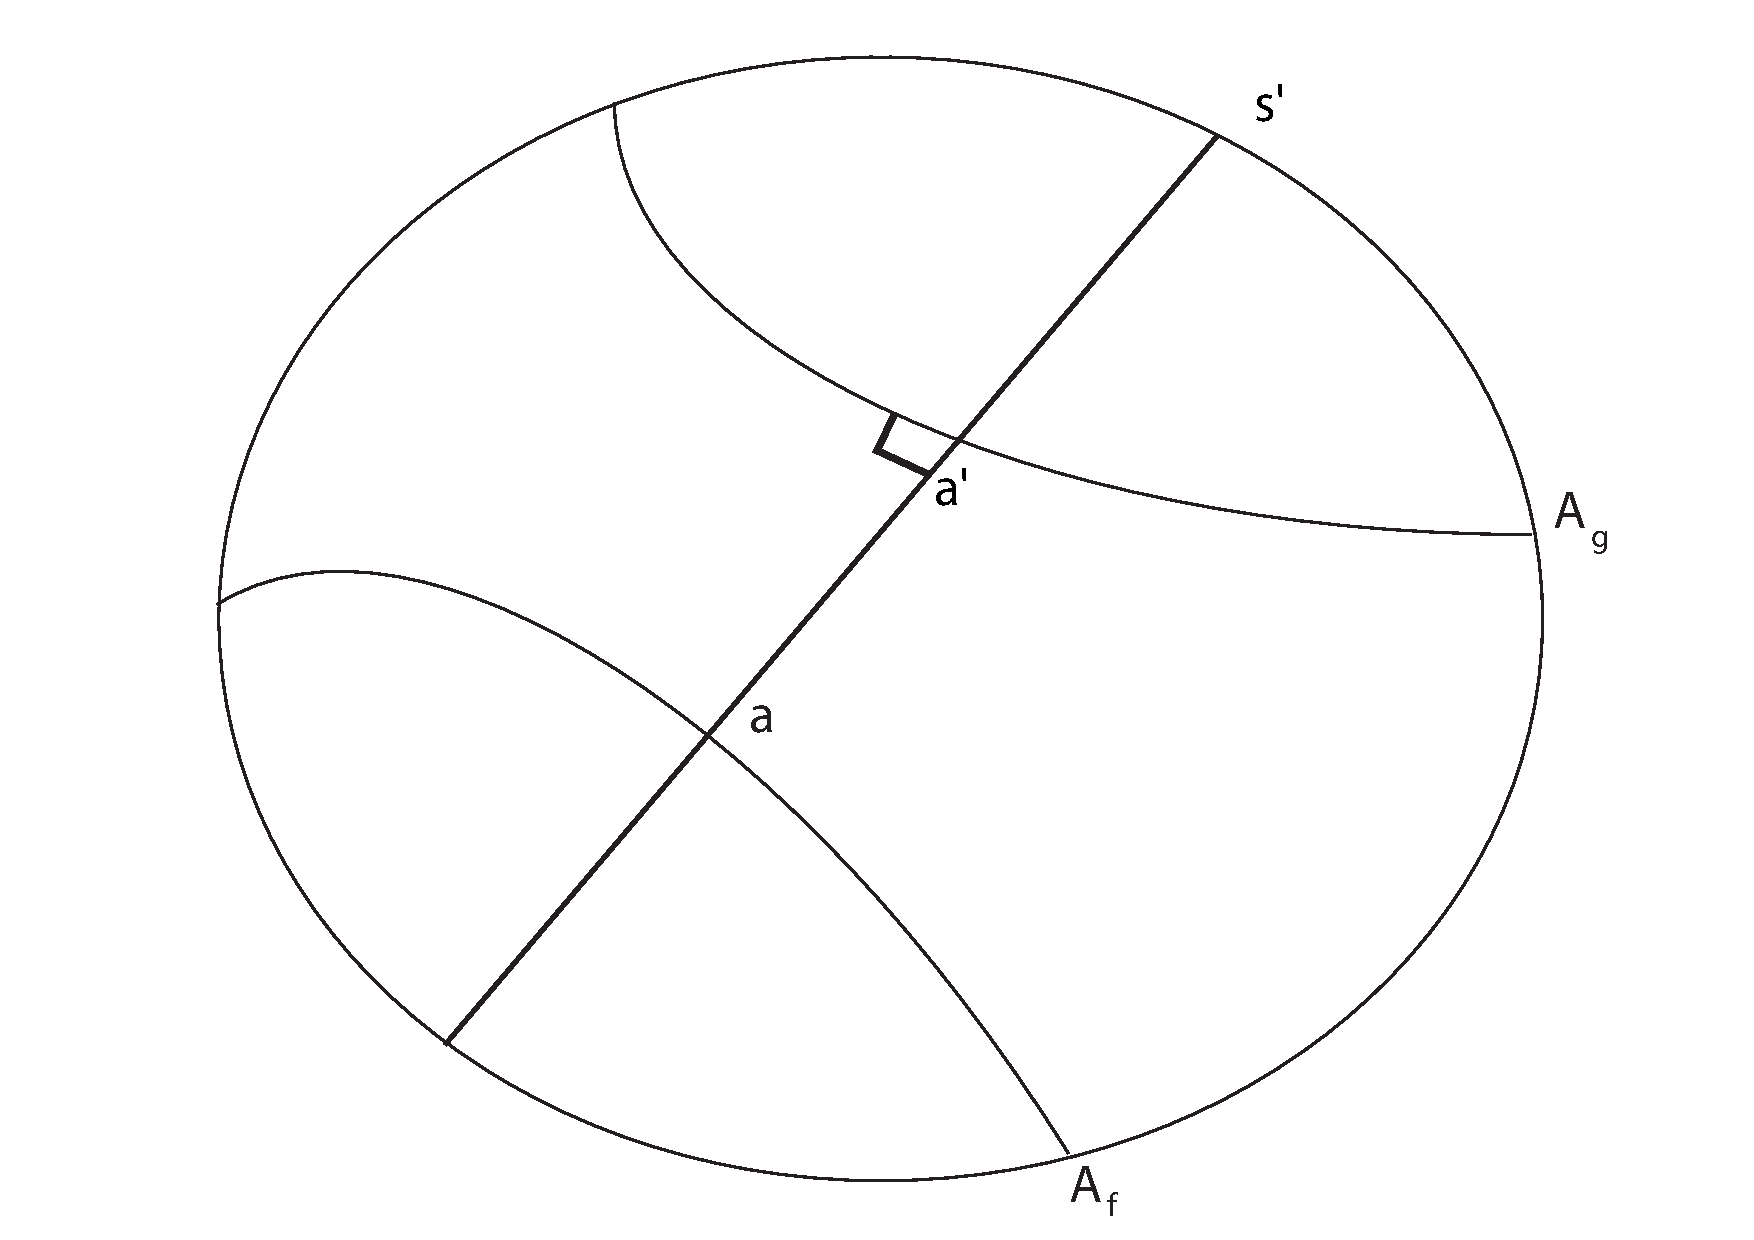
\includegraphics[width=10cm]{lemma1-dem1.pdf}\\
  \caption{Figura \ref{lemma1-dem1} }\label{lemma1-dem1}
\end{figure}


Queremos saber ahora que tipo de transformaci\'on es $fg$, por lo
anterior tenemos que $fg= ss's's'' = ss''$, ahora todo depende de la
posici\'on de los ejes de $f$ y $g$. \\ \\


\textbf{ Caso 1.}[las rectas se intersectan el alg\'un punto de
$D+E$] \\


Sea $m$ el punto medio del segmento $aa'$, la normal a $s'$ que
pasa por $m$ bisecta el \'angulo que forman los ejes en el punto de
intersecci\'on $p$ (\ref{lemma1-dibujo4}), para
ver esto reflejamos las rectas $l$ y $\sigma$ respecto de $l$
obtenemos $l$ y $s''$, como la reflexi\'on es conforme el \'angulo
entre $l$ y $s''$ es el mismo que el \'angulo entre $l$ y $s$. Es
claro que el punto de intersecci\'on $p$ sera el punto fijo de la
transformaci\'on, sea $\frac{1}{2} \phi_{fg}$ el \'angulo entre $s$
y $s'$ (la inversi\'on respecto a dos circunferencias es un elemento el\'iptico con \'angulo el doble del \'angulo de
esta interseccion). \\

\begin{figure}[h]
  \centering
  % Requires \usepackage{graphicx}
  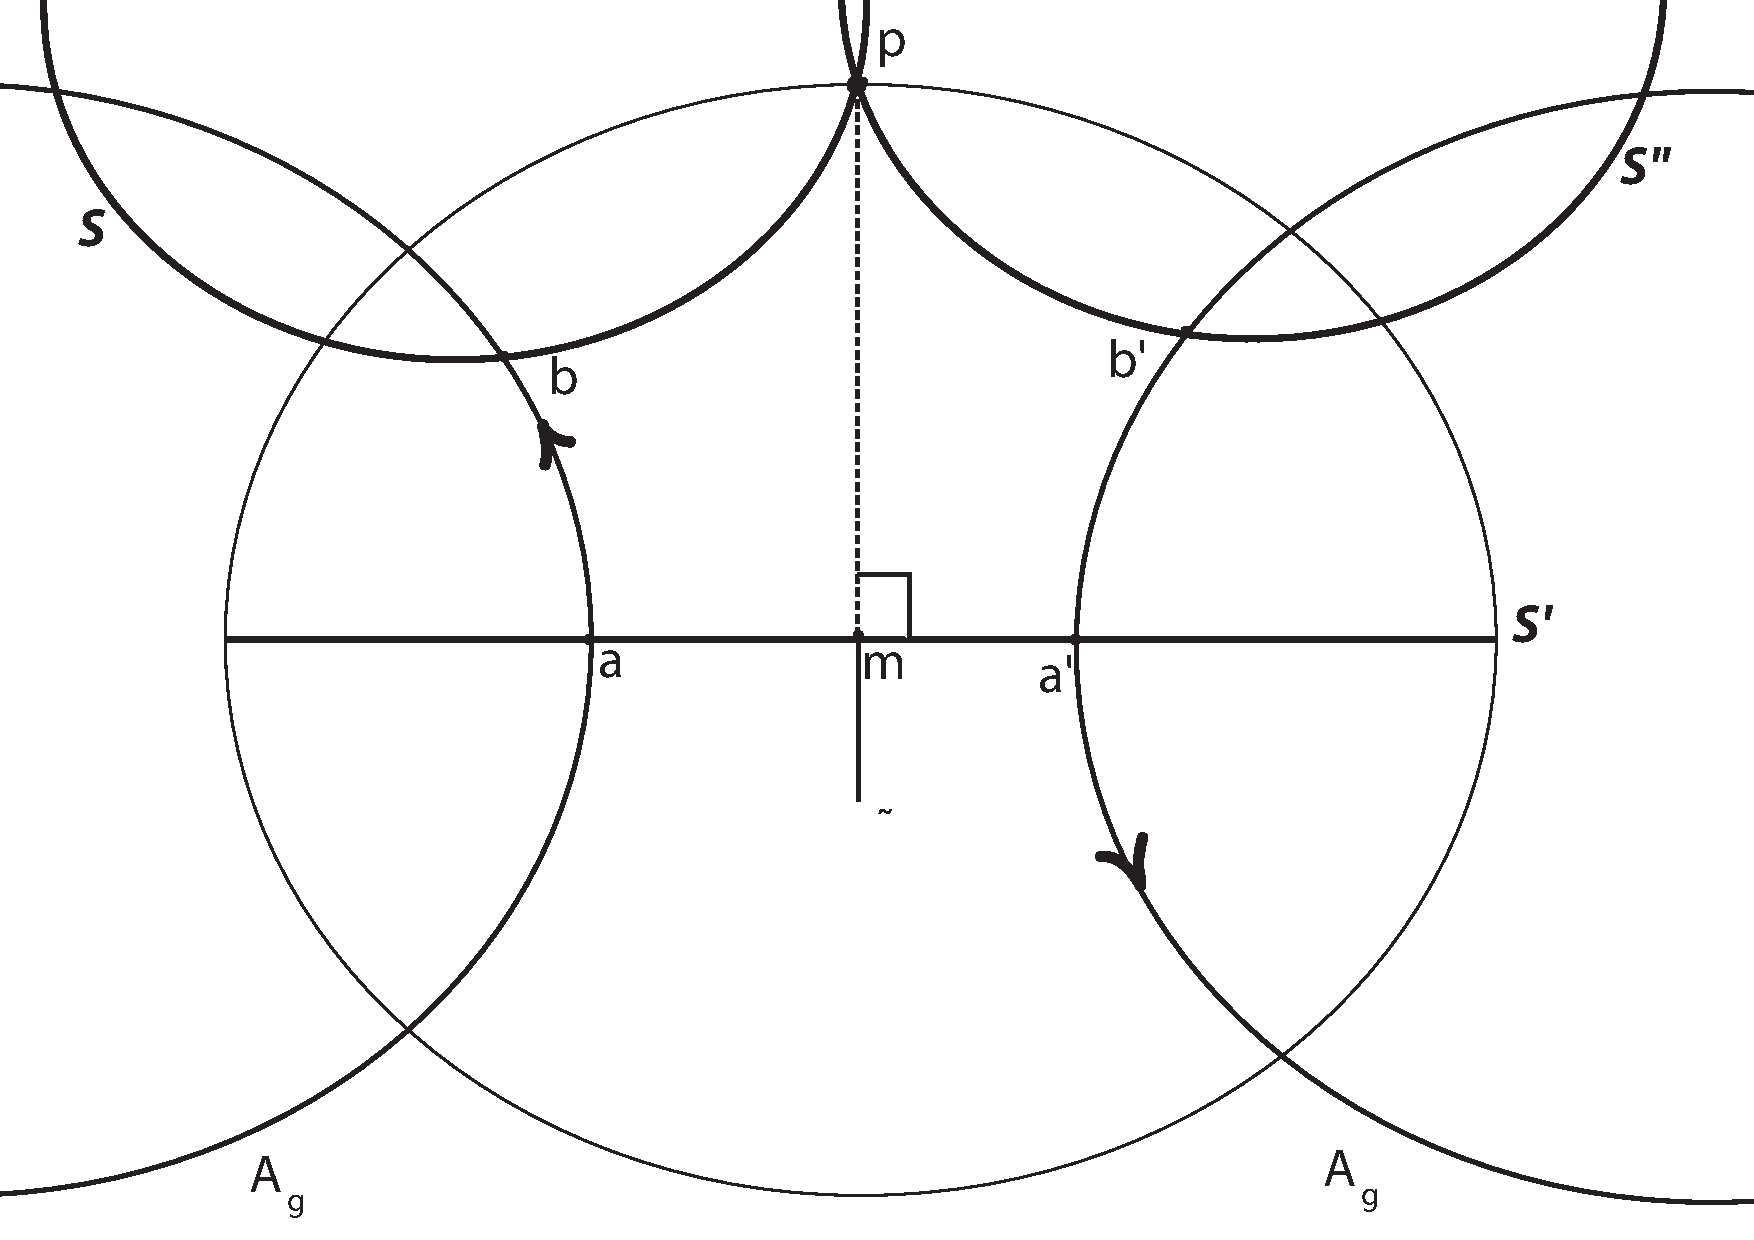
\includegraphics[width=10cm]{lemma1-dibujo4}\\
  \caption{Figura \ref{lemma1-dibujo4}}\label{lemma1-dibujo4}
\end{figure}



Luego $abpm$ es un cuadrilatero con 3 \'angulos rectos y el \'angulo
restante agudo (cuadrilatero de lambert Fig. \ref{lemma1-dibujo5}) cuyas medidas son
$\frac{1}{4} \phi_{fg}$ con lados $\frac{1}{2} \delta$ y $
\frac{1}{2} \lambda$ por lo cual tenemos $senh \frac{1}{2} \delta
senh \frac{1}{2} \lambda = cos \frac{1}{4} \phi_{fg} \leq 1$ y es
igual a 1 en el caso de que se intersecten en el infinito ( $\phi
=0$) y en dado caso la transformaci\'on seria parab\'olica. \\ \\

\begin{figure}[h]
  \centering
  % Requires \usepackage{graphicx}
  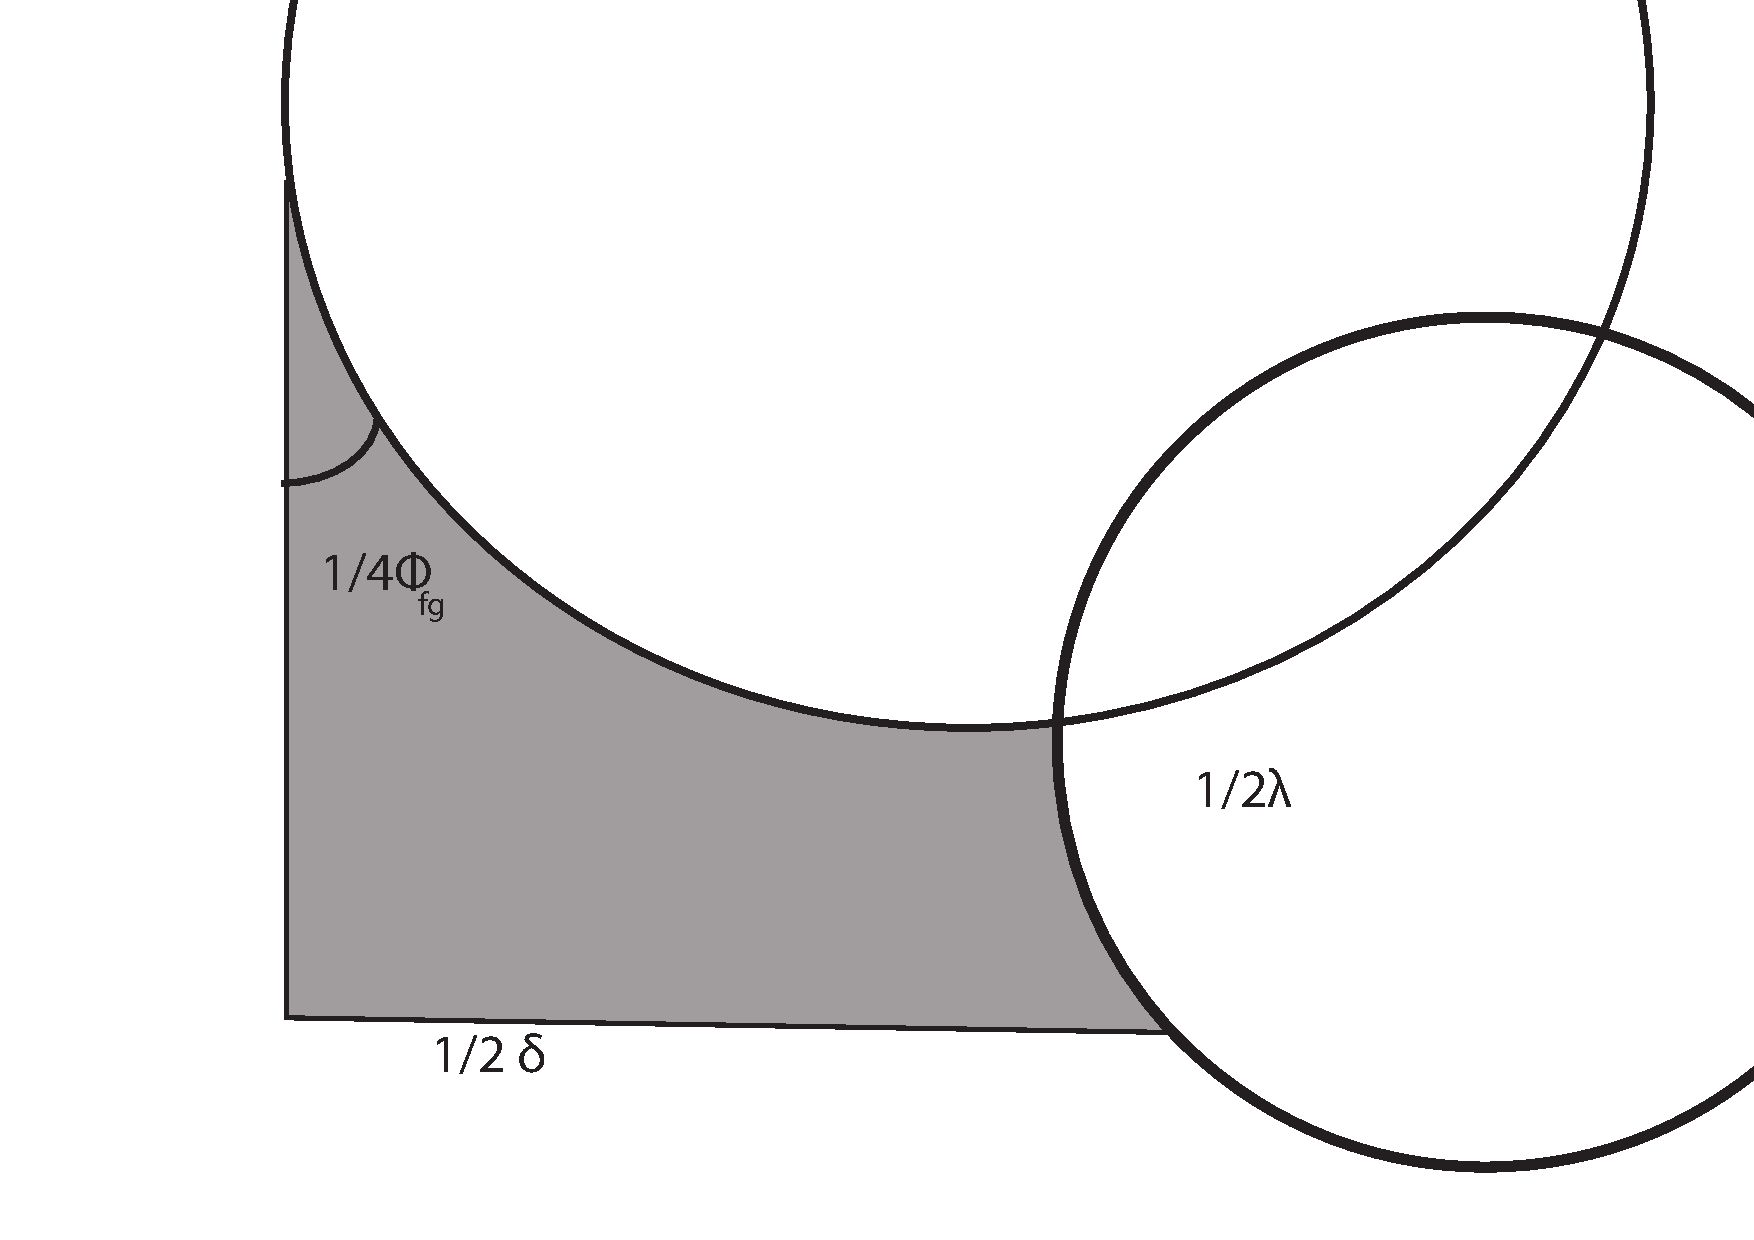
\includegraphics[width=10cm]{lemma1-dibujo5}\\
  \caption{Cuadrilatero de Lambert}  \label{lemma1-dibujo5}
\end{figure}



\textbf{Caso 2}


En el caso que los ejes sean divergentes, existe una recta normal a
ambos  y se tiene que la recta $l$ bisecta al segmento entre $s$ y
$s'$ de esta recta normal, entonces basta probar que;

\begin{enumerate}
\item Esta recta normal es el eje de $fg$
\item En efecto $l$ bisecta al segmento entre $s$ y $s'$ de esta
recta normal
\end{enumerate}

Para (1) Probaremos que $fg$ es hiperb\'olica viendo que tiene dos
puntos fijos y que se encuentran en la normal mencionada antes. Sean
$x$ y $x' $ los puntos finales de dicha recta normal y notemos que
$s''x=x'$ ya que $s''x$ debe cumplir que esta sobre la recta normal
a $s''$ y que $d_{H}(x,s'')=d_{H}(s''x,s'')$ pero $d_{H}(x,s'') =
\infty$, por la misma raz\'on $sx'=x$ entonces $ss''x=x$ y tambien
se cumple $ss''x'=x'$ por lo tanto $fg$ tiene 2 puntos fijos y su
eje es la recta que los une, que en este caso es la recta normal
mencionada (Fig. \ref{lemma1-dibujo6-2}).

\begin{figure}[h]
  \centering
  % Requires \usepackage{graphicx}
  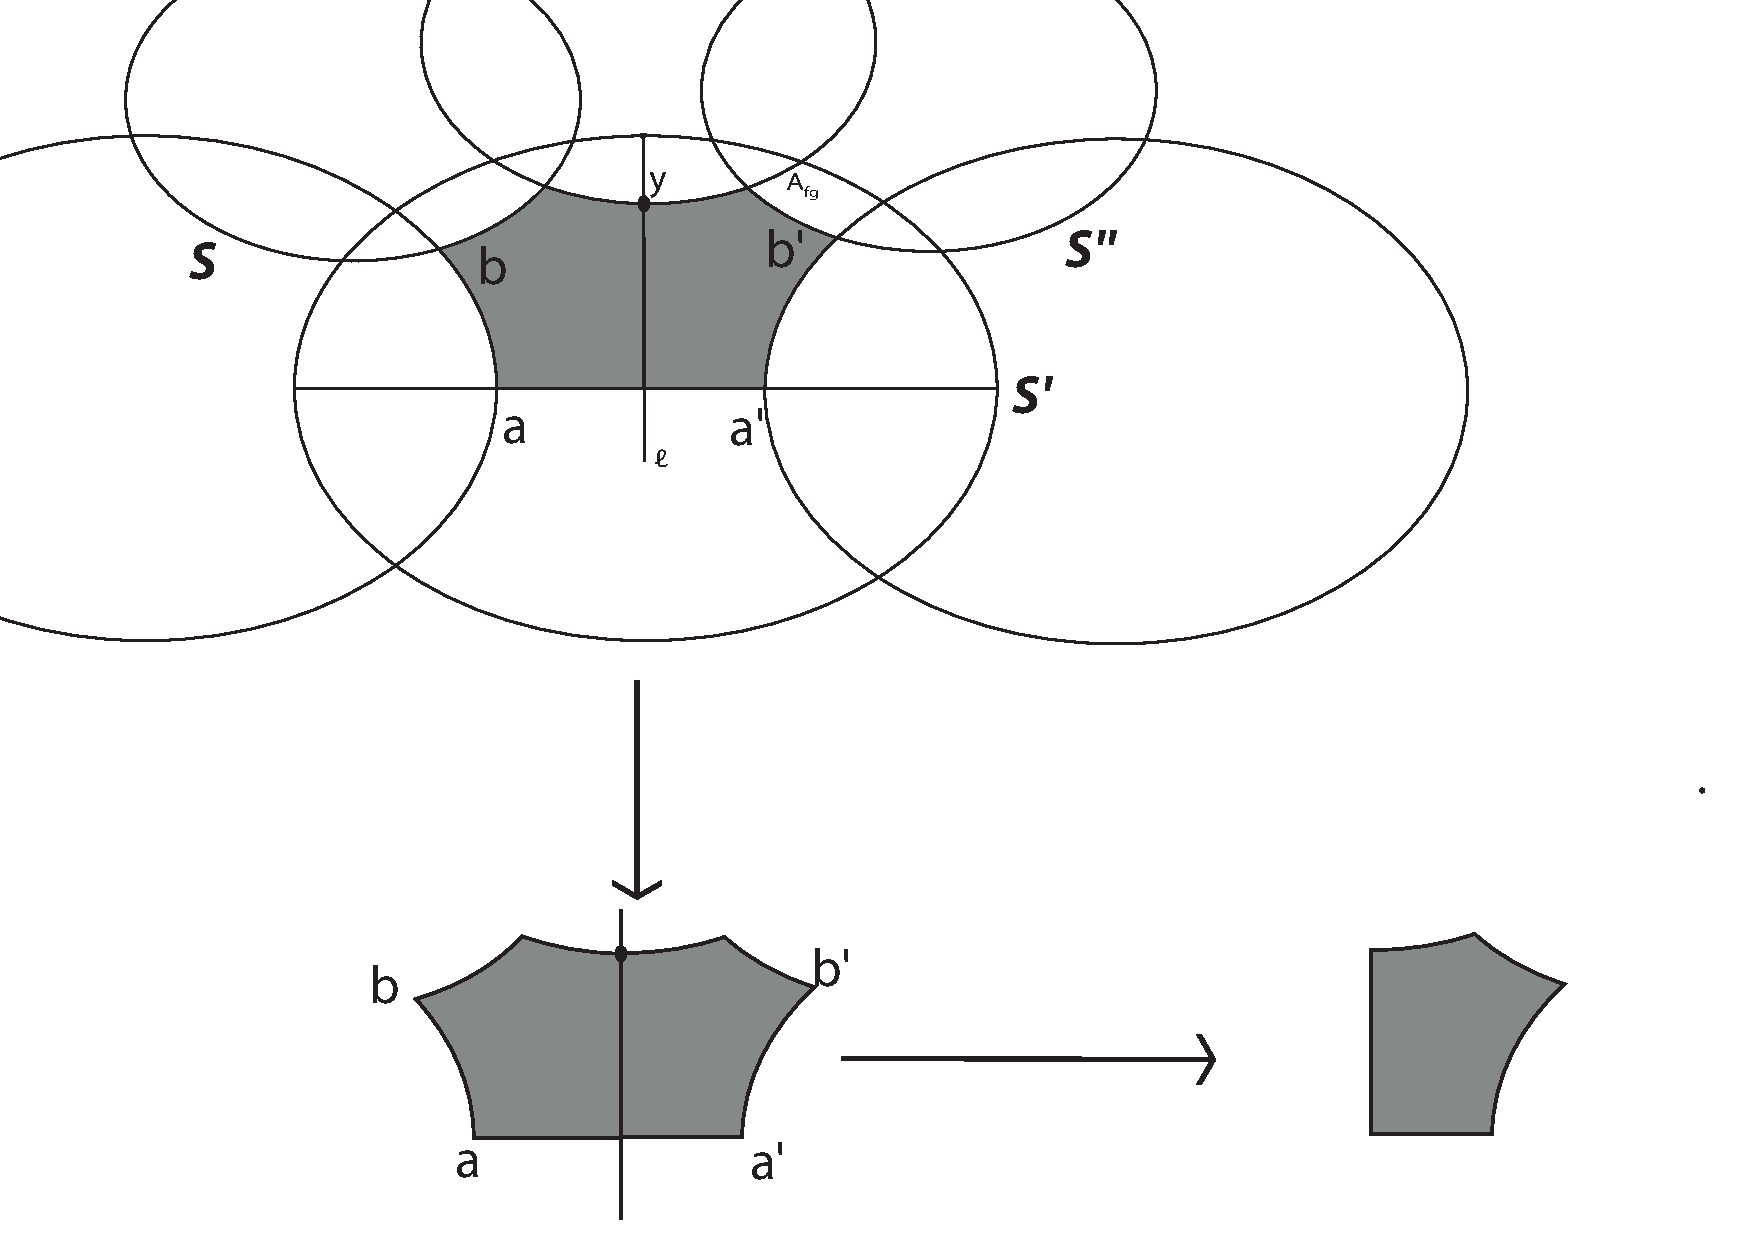
\includegraphics[width=10cm]{lemma1-dibujo6-2}\\
  \caption{Figura \ref{lemma1-dibujo6-2} }\label{lemma1-dibujo6-2}
\end{figure}


Para (2) queremos probar que $d_{H}(x,y) = d_{H}(y,x')$ donde $y$ es
el punto de intersecci\'on de la normal con $l$, al reflejar
respecto de $l$ y notando que $x \mapsto x'$ bajo $s$ y $d_{H}(x,y)
= d_{H}(y,sx)$ tenemos el resultado. \\


Finalmente tenemos las rectas $s'',A_{g},s,l$ y $A_{fg}$ y estas
forman un pentagono con 4 \'angulos rectos y con lados
$\frac{1}{2}\lambda_{fg},\frac{1}{2}\delta,\frac{1}{2}\lambda$
 (Fig. \ref{lemma1-dibujo9}) y podemos concluir (\ref{cha:apendice})
$$ senh \frac{1}{2} \delta senh \frac{1}{2} \lambda = cosh \frac{1}{4} \lambda_{fg} >1$$
$ _{\square} $

\begin{figure}[h]
  \centering
  % Requires \usepackage{graphicx}
  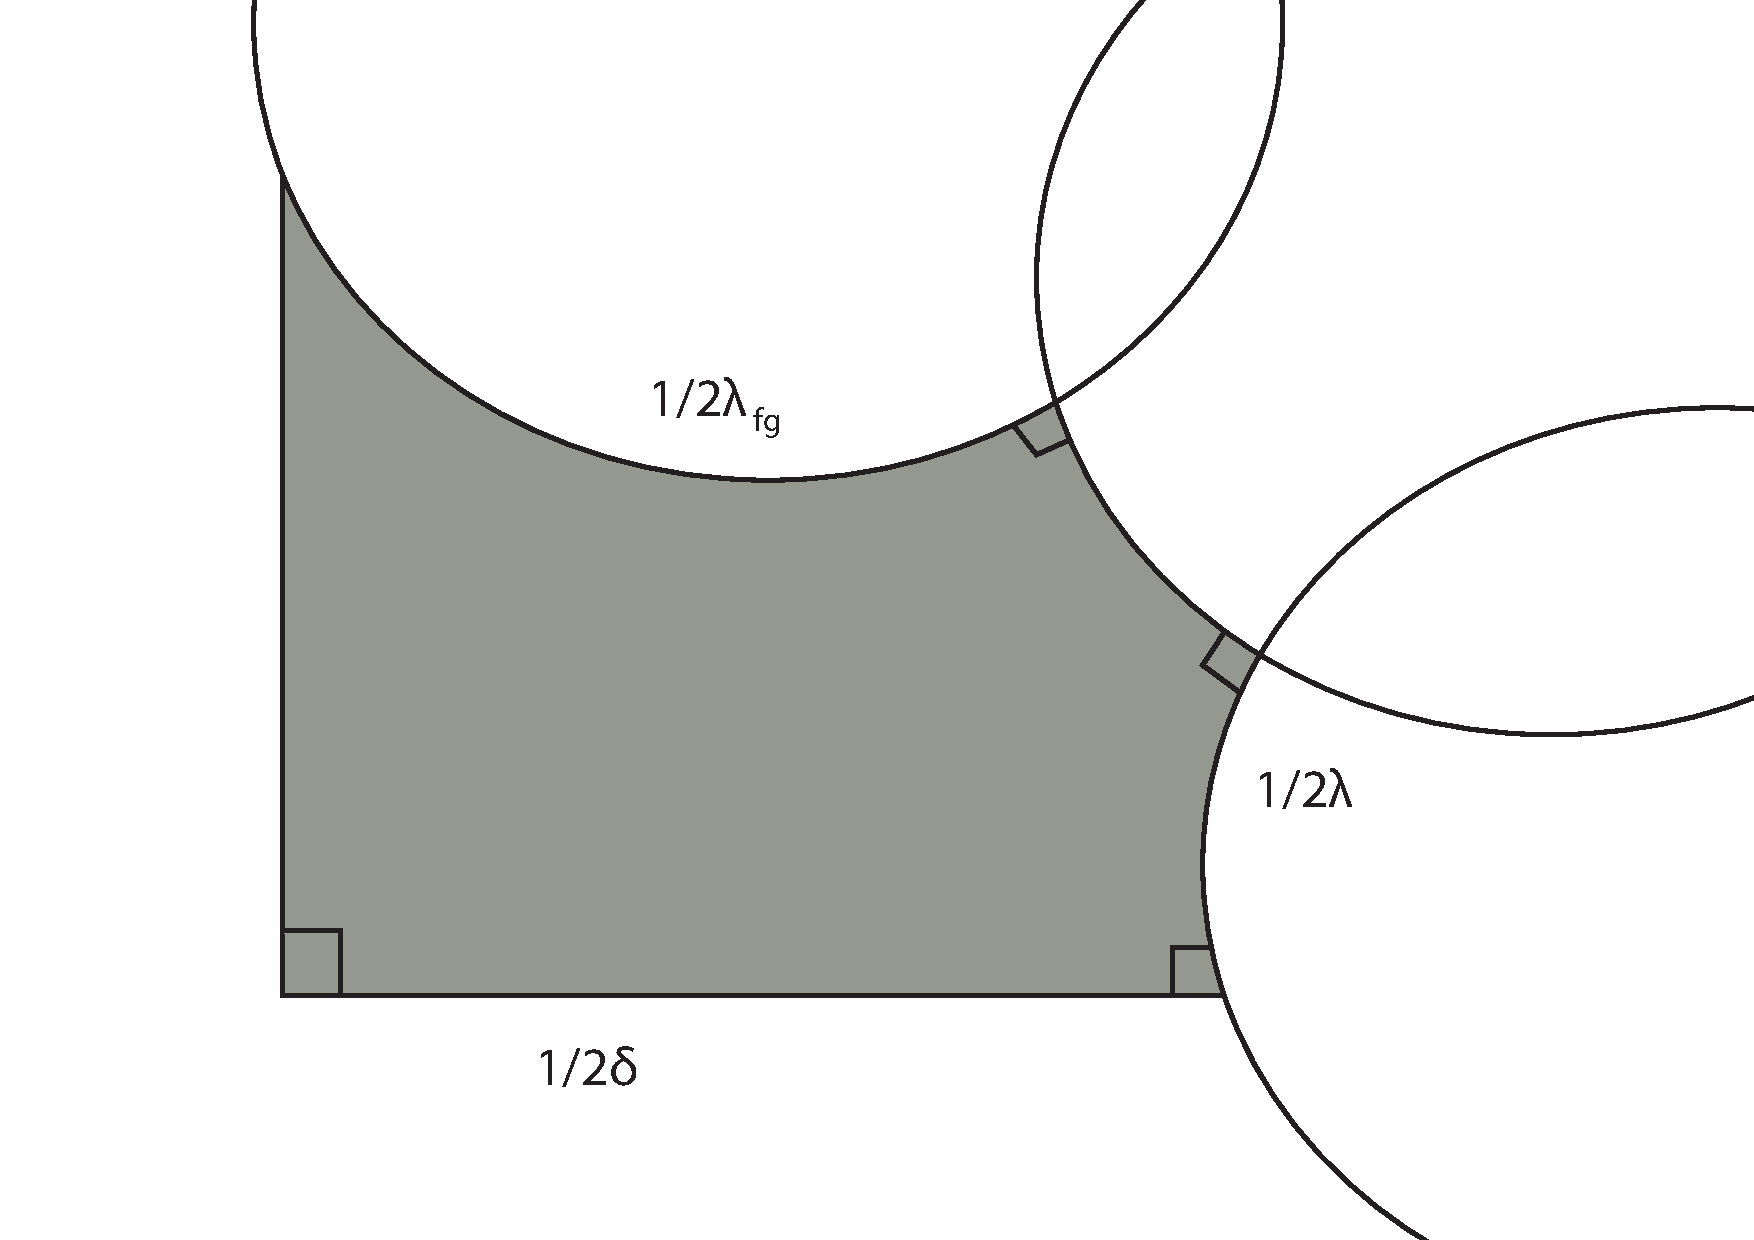
\includegraphics[width=10cm]{lemma1-dibujo9}\\
  \caption{Pent\'agono con 4 \'angulos rectos}\label{lemma1-dibujo9}
\end{figure}



\section{El lema del conmutador de los elemetos hiperb\'olicos}

\begin{lem} \label{lema2}
Sean $f$ y $g$ dos elementos hiperb\'olicos con ejes $A_{f}$ y
$A_{g}$ y desplazamientos iguales $\lambda $, y con \'angulo de
intersecci\'on $\phi $.El conmutador $[f,g]=fgf^{-1}g^{-1}$
es el\'iptico , parab\'olico o hiperb\'olico dependiendo de

$$ senh^{2}(\frac{1}{2} \lambda) sen \phi  \left \{ \begin{matrix} >1
\\ =1 \\ < 1 \end{matrix}\right. $$
\end{lem}

\textit{Prueba}:

Sea $s'$ el punto de intersecci\'on de $A_{f}$  y $A_{g}$, sea $s$
el punto sobre $A_{f}$ tal que $d_{H}(s',s)= \frac{1}{2} \lambda$ y
trazado siguiendo la direcci\'on de $A_{f}$, y sea $s''$ el punto
sobre $A_{g}$ tal que $d_{H}(s',s'')=\frac{1}{2} \lambda$ y trazado
siguiendo la misma direcci\'on que $A_{g}$ (Fig. \ref{lemma2-dibujo1}). \\

\begin{figure}[h]
  \centering
  % Requires \usepackage{graphicx}
  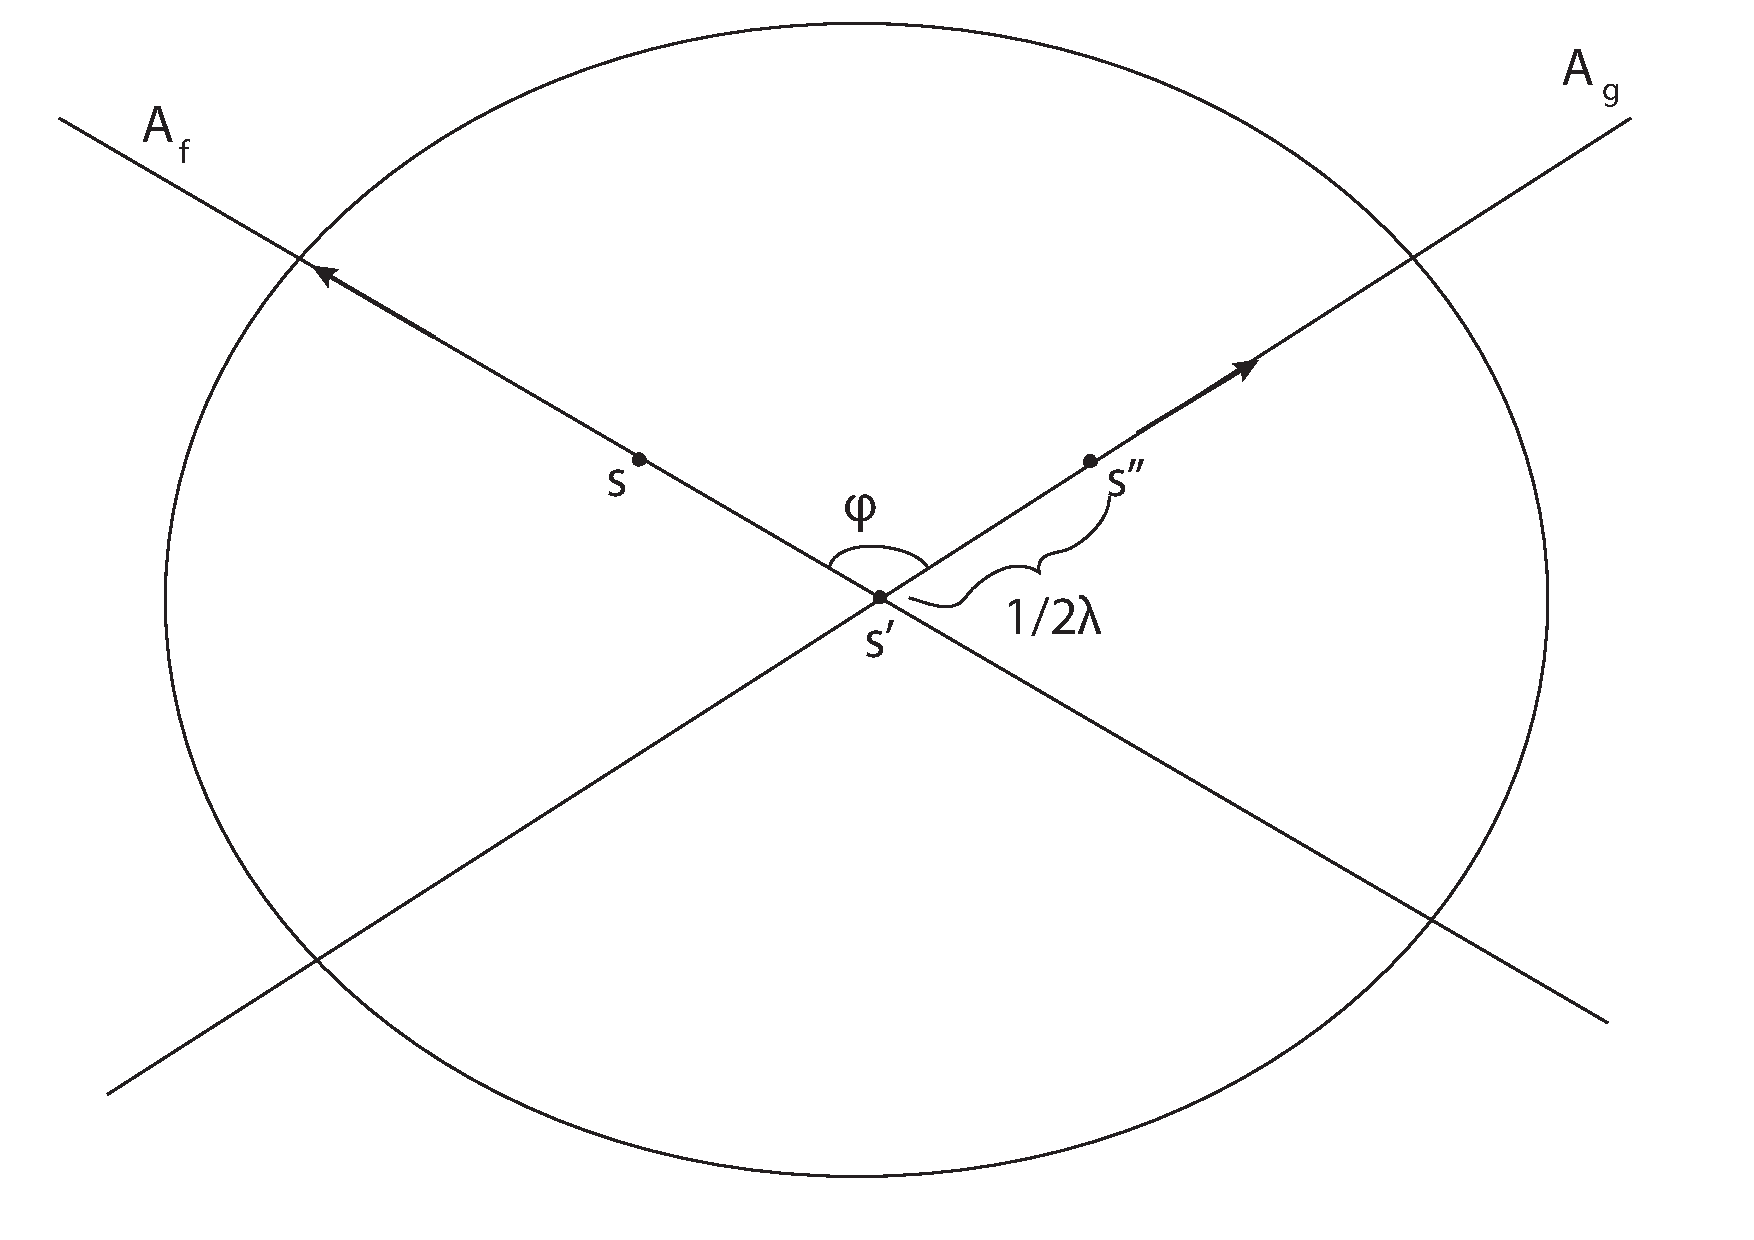
\includegraphics[width=10cm]{lemma2-dibujo1}\\
  \caption{Figura \ref{lemma2-dibujo1}}\label{lemma2-dibujo1}
\end{figure}


Y consideremos los elementops el\'ipticos de \'angulo $\pi$  respecto a estos puntos
y los denotaremos igual que denotamos a sus puntos fijos. \\

Queremos primero probar que $f=ss'$, para esto deseamos ver los puntos que deja fijos $ss'$. El elemento el\'iptico con \'angulo $\pi$ funciona de la
siguiente manera; dado un punto $x$ se traza la recta que va de $x$
al punto fijo $c$,la im\'agen de $x$ bajo el elemento el\'iptico llamemosle $y$ esta
sobre la misma recta y $d_{H}(x,c)=d_{H}(y,c)$, con este proceso
podemos ver que $ss'$ fija los mismos puntos que $f$ por lo tanto el
eje de $f$ es el mismo que el  de $ss'$ solo falta ver cuanto es el
desplazamiento de $ss'$,como antes, basta verificarlo para un
punto y en esta ocasi\'on tomamos el punto $s'$, tenemos que
$d_{H}(s,ss'(s'))=d_{H}(s,s(s'))= 2d_{H}(s',s)=2(\frac{1}{2}
\lambda)= \lambda $ por lo tanto $f=ss'$. Un proceso an\'alogo nos
enseña que $g=s's''$ y como $s's'$ es la indentidad entonces $fg
= ss''$, m\'as a\'un $f^{-1} = s's,g^{-1}=s''s'$ y entonces
$f^{-1}g^{-1}= s'ss''s'=s'fgs'=s'fgs'^{-1}$, luego $ss'$ es un
elemento hiperb\'olico con recta invariante igual a la recta que pasa por
$s$ y $s''$ y desplazamiento $2d_{H}(s,s'')$, m\'as a\'un
$f^{-1}g^{-1}$ es hiperb\'olico obtenido de $fg$ conjungando por
$s'$, tenemos entonces;

\begin{enumerate}
\item $f^{-1}g^{-1}$ tiene un desplazamiento con la misma medida que
$fg$
\item su eje $A_{f^{-1}g^{-1}}$ se obtiene de $A_{fg}$ rotando por $s'$.
\end{enumerate}

Para probar (1) queremos ver cuanto mide $d_{H}(x,s'fgs'x)$ y
tenemos que $d_{H}(x,s'fgs'x)= d_{H}(s'x,fg(s'x))$ y esta \'ultima
cantidad es el desplazamiento de $fg$. \\ \\

(2) se cumple  ya que $f^{-1}g^{-1} (s'A_{fg})= s'fgs'(s'A_{fg})=
s'fg(A_{fg})=s'A_{fg}$. \\

Entonces estos ejes son divergentes y sus correspondientes
transformaciones tienen sentidos opuestos, aplicamos entonces el
\textbf{lema} \ref{lema1} a $fg$ y a $f^{-1}g^{-1}$ entonces $[f,g]$ es
el\'iptico , parab\'olico o hiperb\'olico seg\'un sea

$$senh \eta senh \frac{1}{2} \lambda_{fg} \lesseqgtr 1$$

Donde $\eta$ es la perpendicular desde $s'$ en el tri\'angulo
$ss's''$ (Fig. \ref{lemma2-dibujo4}) y por trigonometr\'ia hiperb\'olica (\ref{cha:apendice}) se cumple $senh \eta
senh\frac{1}{2} \lambda_{fg} = sen \phi senh^{2} \frac{1}{2}\lambda$
$_{\square}$

\begin{figure}[h]
  \centering
  % Requires \usepackage{graphicx}
  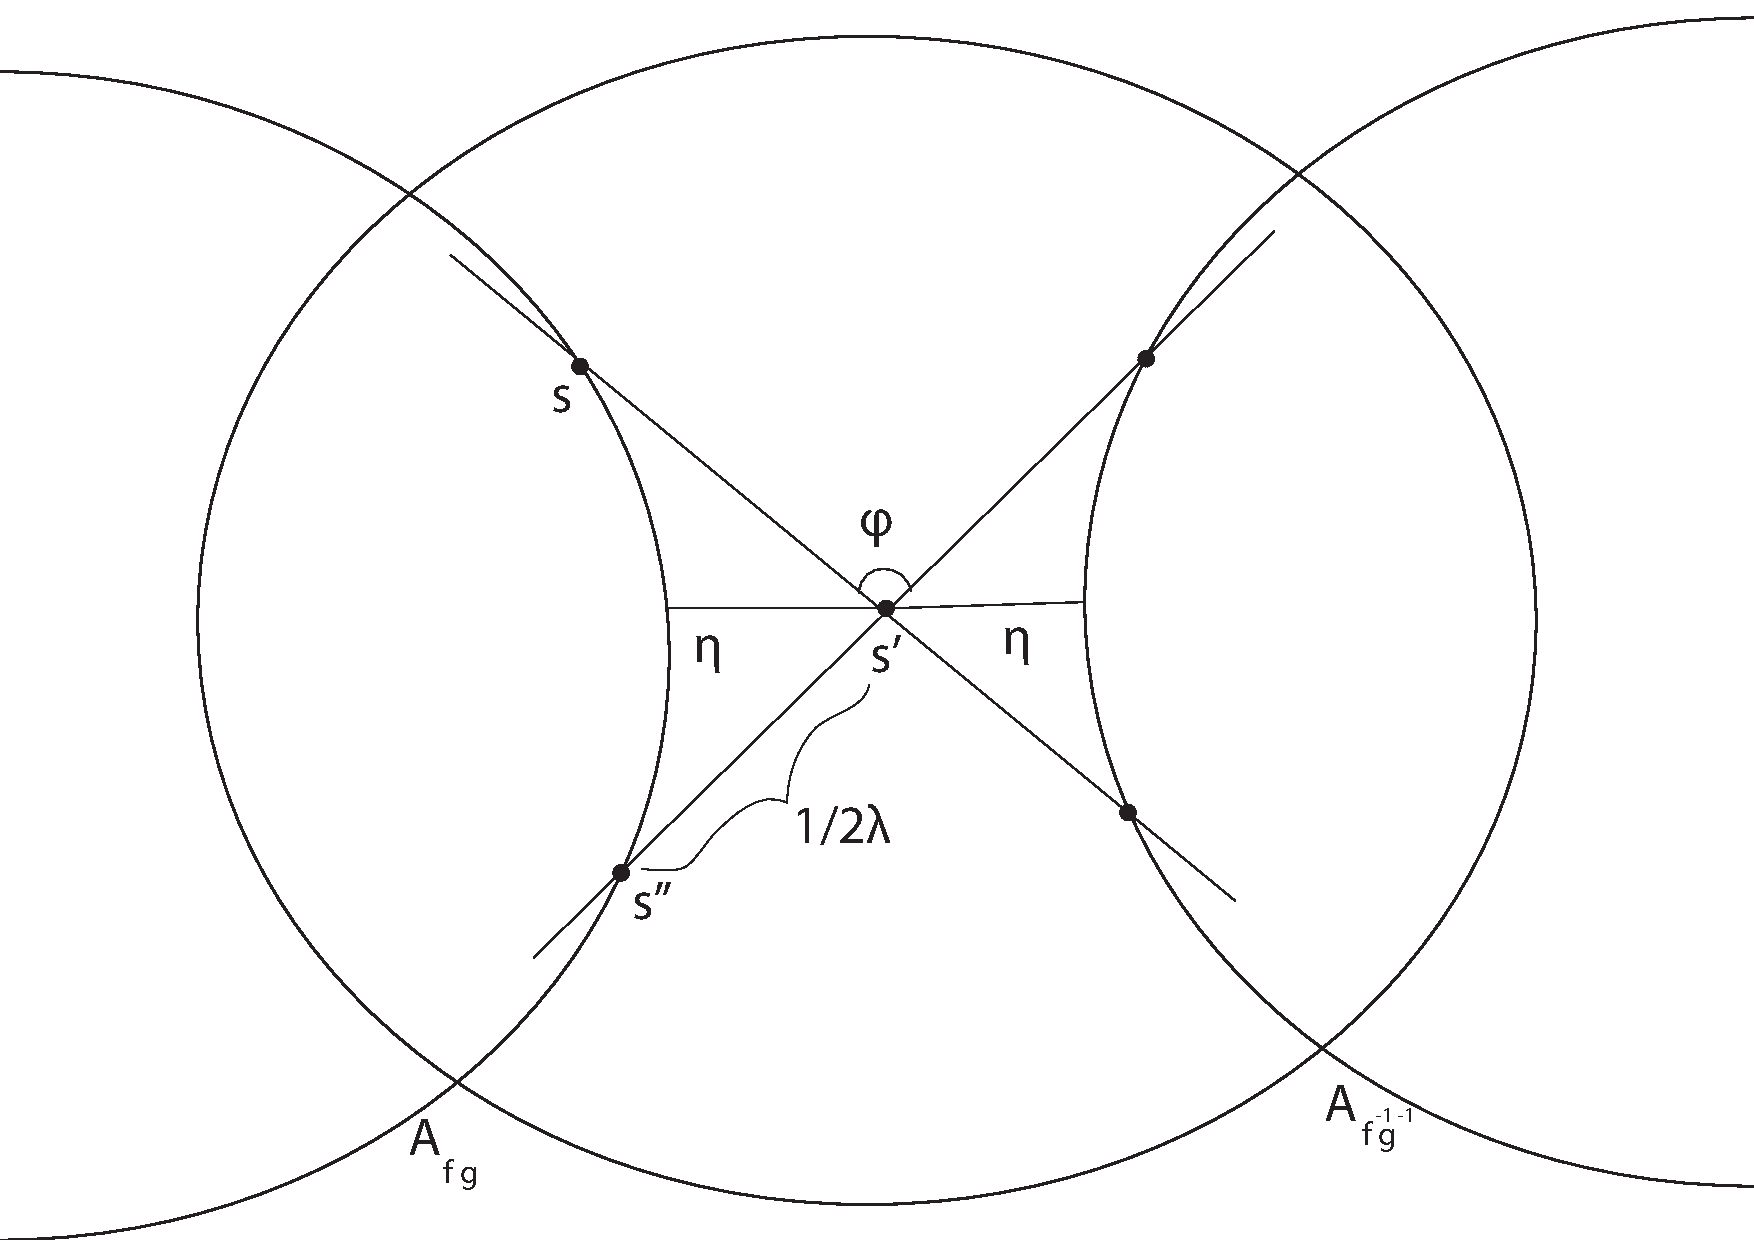
\includegraphics[width=7cm]{lemma2-dibujo4}\\
  \caption{Figura \ref{lemma2-dibujo4}}\label{lemma2-dibujo4}
\end{figure}


\section{El lema del conmutador de los elementos parab\'olicos}

\begin{lem}\label{lema3}
Sean $f,g$ elementos parab\'olicos con puntos fijos $c_{f}$ y
$c_{g}$ entonces el conmutador $[f,g]$ es hiperb\'olico.
\end{lem}

\emph{Prueba.} \\

\begin{figure}[h]
  \centering
  % Requires \usepackage{graphicx}
  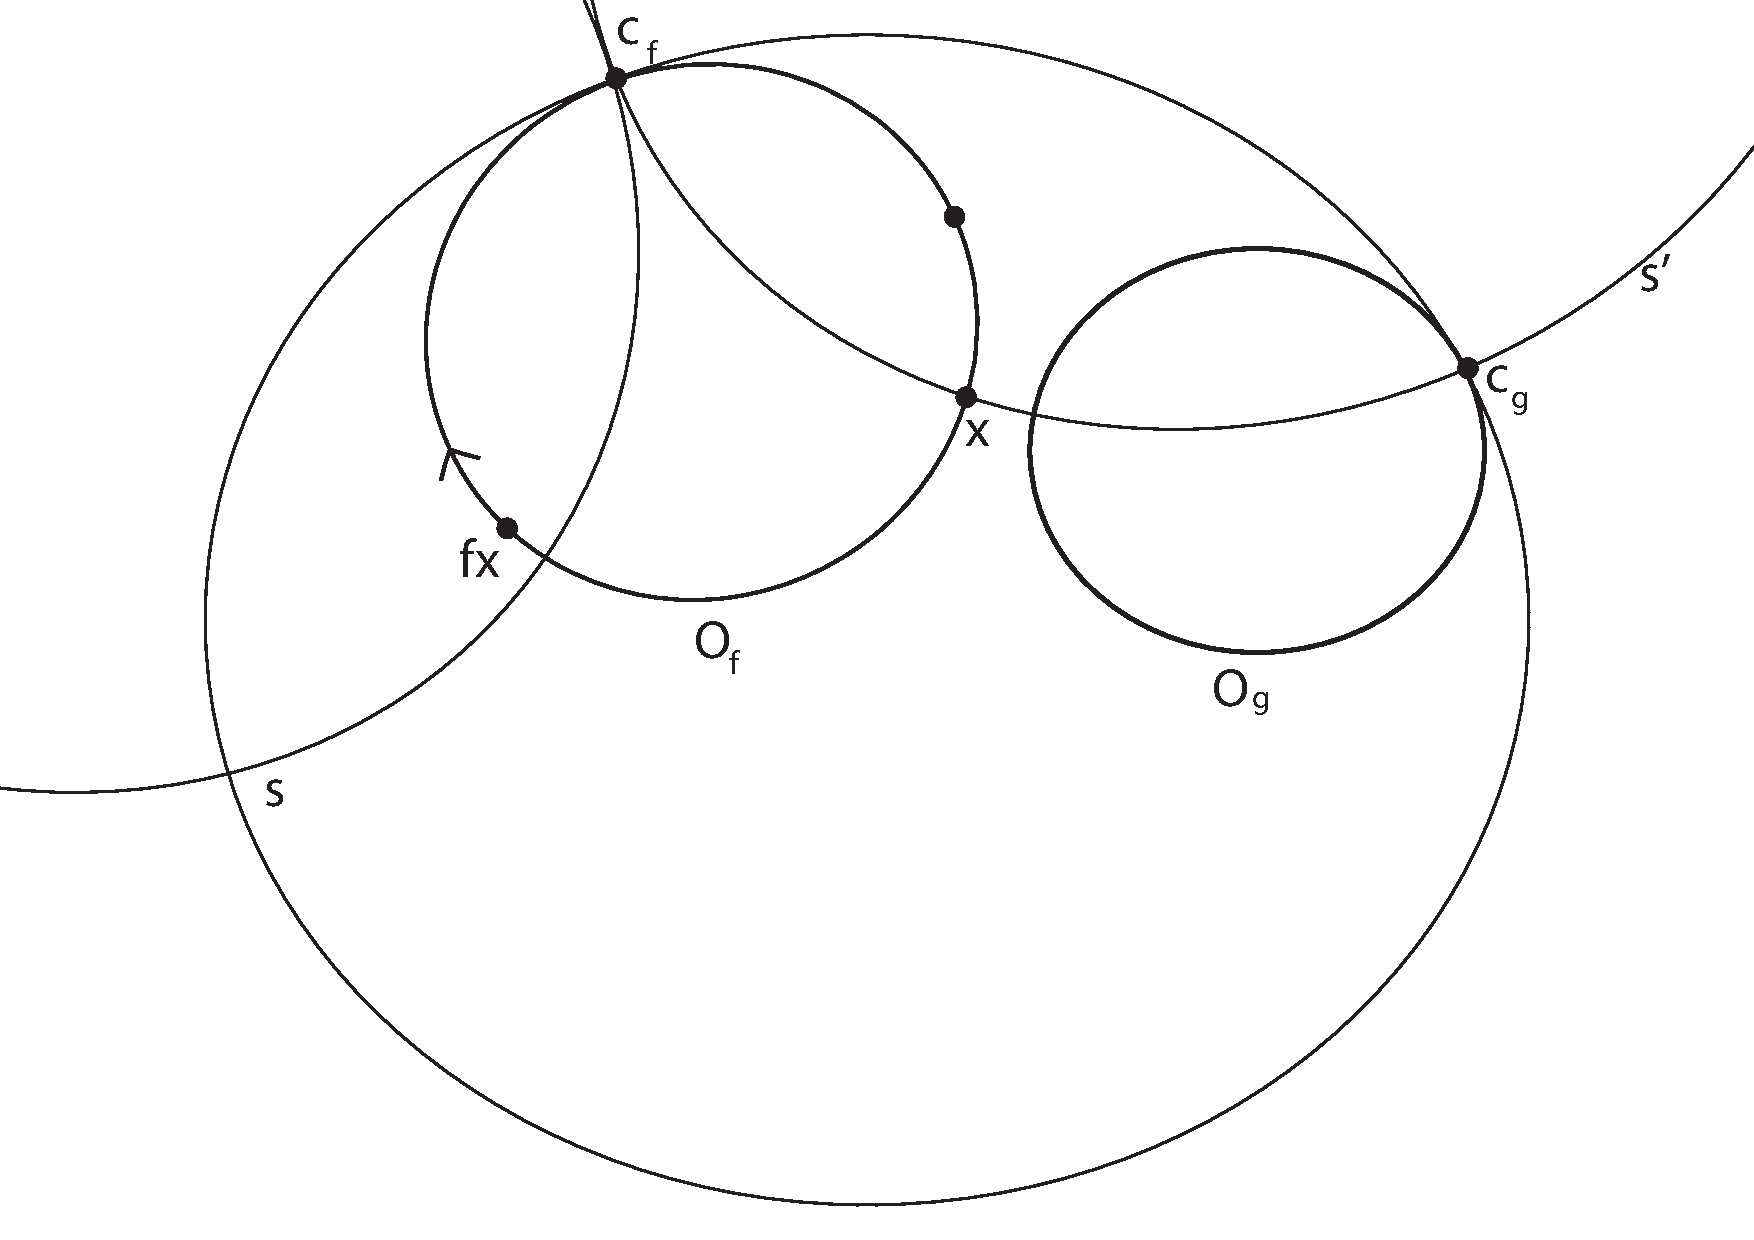
\includegraphics[width=10cm]{lemma3-dibujo1}\\
  \caption{Figura \ref{lemma3-dibujo1}}\label{lemma3-dibujo1}
\end{figure}


 Sea $s'$ la recta que une $c_{f}$ y $c_{g}$ y denotemos la reflexi\'on respecto a esta recta
tambi\'en como $s'$. Sea $O_{f}$ un horociclo dado con punto al
infinito $c_{f}$, y $x \in O_{f}$, tomamos $s$ en el conjunto de geod\'esicas que pertenece al haz parab\'olico con punto fijo $c_{f}$ (\cite{Beardon}).

Tenemos entonces que $ f=ss' $, y analogamente obtenemos  que existe
$s''$ tal que $g=s's''$ luego tenemos
$[f,g]=ss''s'ss''s'=(ss''s')^{2}$, la composici\'on de reflexiones
conserva el sentido por lo tanto la composici\'on de 3 reflexiones
invierte el sentido y es por tanto una reflexi\'on o una
h-reflexi\'on entonces su cuadrado es la identidad o un elemento
hiperb\'olico.Probemos que  $f$ y $g$ no permutan: Si $fg=gf$, tenemos que $f$ deja invariante el conjunto de puntos fijos de $g$ y vicerversa, para ver esto sea $x$ un punto fijo de $f$ entonces $f(g(x))= g(f(x)) = g(x)$, es decir $g(x)$ es un punto fijo de $f$, si sustituimos $g$ por $g^{-1}$ analogamente obtenemos que $g^{-1}(x)$ es un punto fijo, es decir todo punto fijo es la imagen bajo $g$ de otro punto fijo ( $x= g(g^{-1}(x))$). Dado esto $[f,g]$ es la identidad si y solo si $f$ y $g$ conmutan, como hemos probado que esto no es posible se tiene que $[f,g]$ es un elemento hiperb\'olico. $_{\square}$

\section{El lema del conmutador de los elementos hiperb\'olicos con ejes paralelos}

\begin{lem} \label{lema4}
Sean $f$ y $g$ elementos hiperb\'olicos con ejes paralelos y con
punto com\'un $u$, entonces el conmutador $[f,g]$ es un elemento
parab\'olico con centro en $u$
\end{lem}

\begin{figure}[h]
  \centering
  % Requires \usepackage{graphicx}
  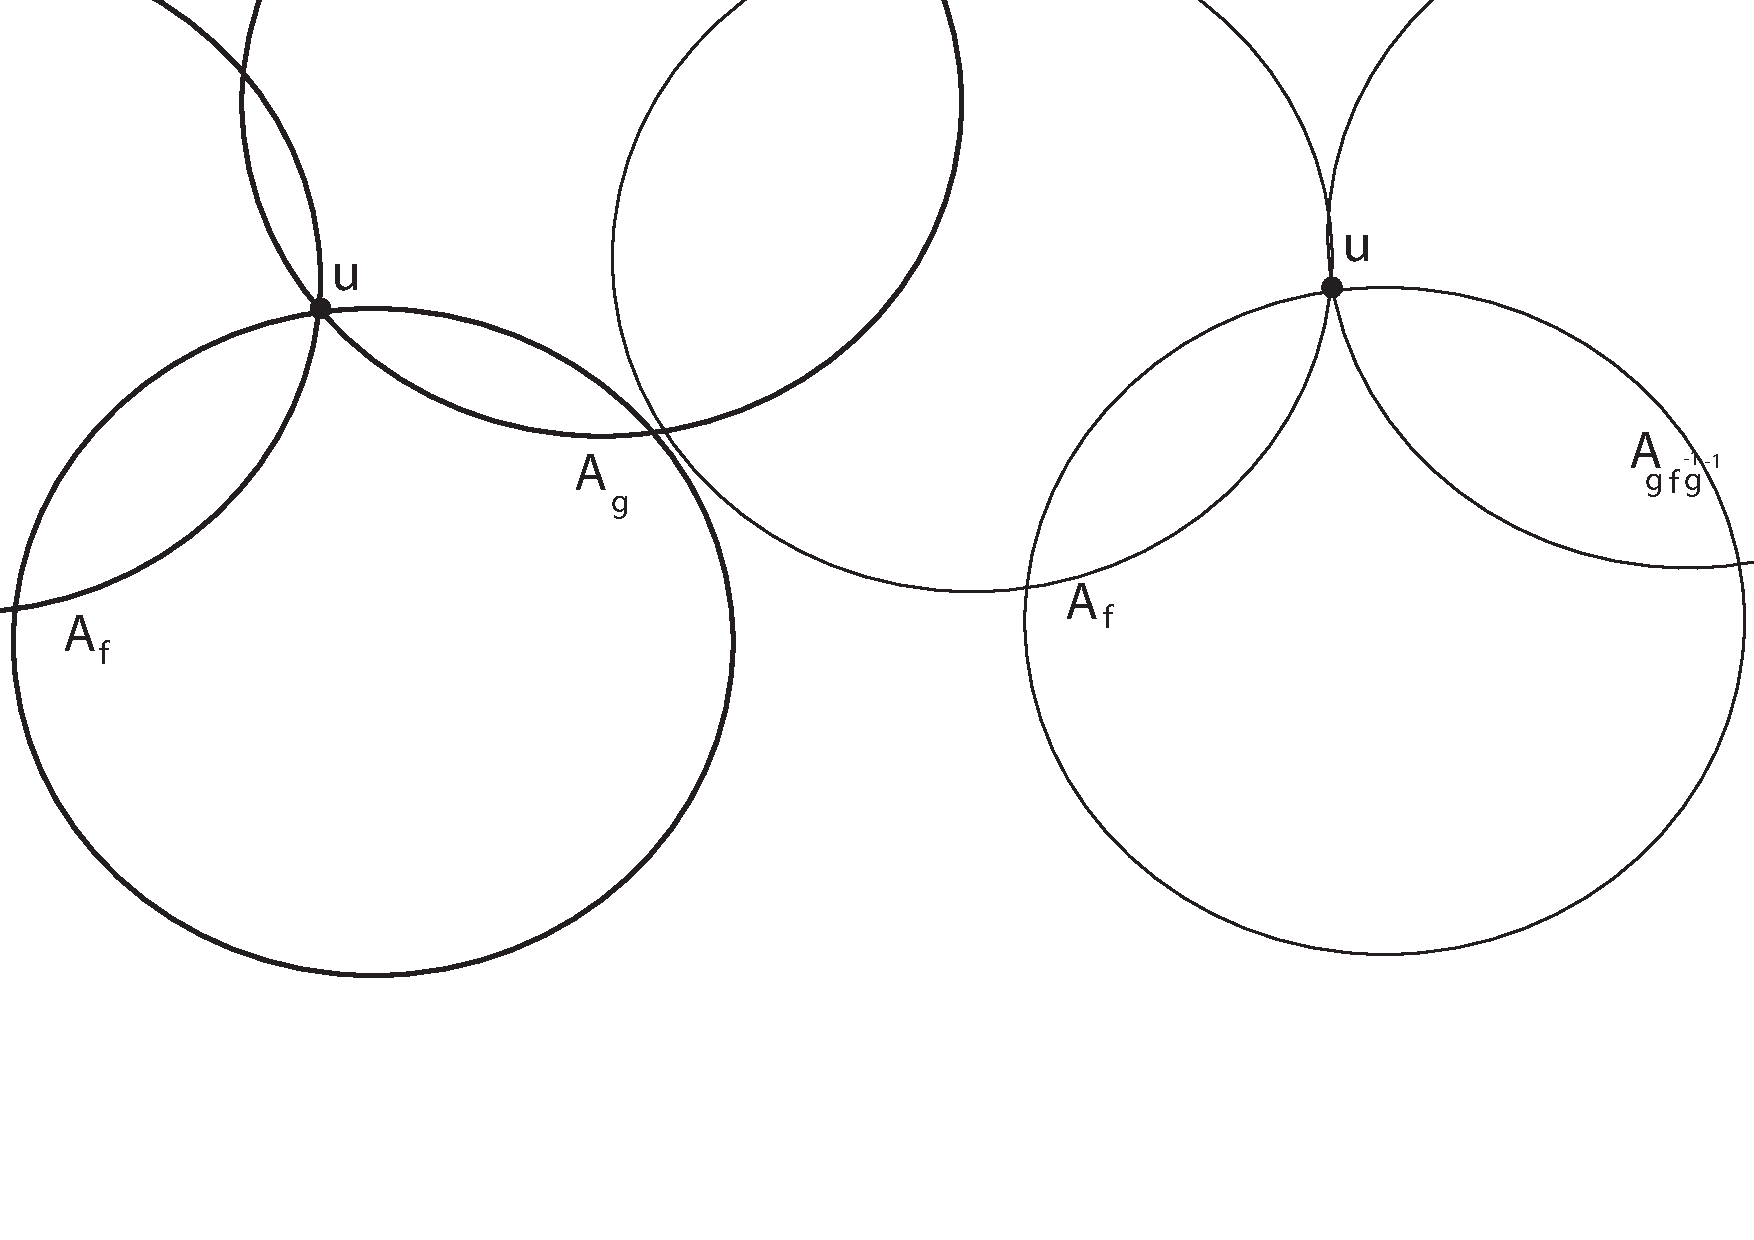
\includegraphics[width=10cm]{lemma4-dibujo1}\\
  \caption{Figura \ref{lemma4-dibujo1}}\label{lemma4-dibujo1}
\end{figure}



\textit{Prueba}:

Primero veamos que  $f \neq gf^{-1}g^{-1}$, es claro que
$gf^{-1}g^{-1}$ fija $u$ ya que tanto $f$ como $g$ lo fijan, sea $x$
el punto final del eje de $f$ distinto de $u$, es claro que $g^{-1}$
no fija este punto, y $gx \neq u$ (puesto que $g^{-1}u \neq x$)
concluimos con esto $f \neq gf^{-1}g^{-1}$.

Sin perdida de generalidad podemos suponer que $u=0$ y que las matrices de los elementos hiperb\'olicos correspondientes a $f$ y $g$ lucen de la siguiente manera:

$$M_{f}=    \begin{pmatrix}
 a& 0\\
 c & d
 \end{pmatrix} \  ,  \ M_{g} =     \begin{pmatrix}
 x& 0\\
 w& z
 \end{pmatrix}   $$

 Donde $ad=1,xz=1$ , $|a+d|>2$ y $|x+z|>2$. Haciendo los c\'alculos obtenemos que $tr (M_{f}M_{g}M_{f^{-1}}M_{g^{-1}})=2$ por lo que el conmutador es un elemento parab\'olico con punto fijo $u=0$. $_{\square}$

%Primero veamos que  $f \neq gf^{-1}g^{-1}$, es claro que
%$gf^{-1}g^{-1}$ fija $u$ ya que tanto $f$ como $g$ lo fijan, sea $x$
%el punto final del eje de $f$ distinto de $u$, es claro que $g^{-1}$
%no fija este punto, y $gx \neq u$ (puesto que $g^{-1}u \neq x$)
%concluimos con esto $f \neq gf^{-1}g^{-1}$, claramente su
%desplazamiento mide lo mismo (debido a que $g$ es isometria) pero
%con sentidos opuestos (ya que $gf^{-1}g^{-1}$ respeta el sentido de
%$f^{-1}$). (\textcolor[rgb]{1.00,0.00,0.00}{dibujo})
%(\textcolor[rgb]{0.00,0.00,1.00}{inconcluso}).

\section{El lema del elemento el\'iptico}

\begin{lem} \label{lema5}
Si en un grupo $G < PSL(2,\mathbb{R})$ sin puntos invariantes, 2
ejes de elementos hiperb\'olicos son paralelos entonces el grupo
contiene un elemento el\'iptico
\end{lem}


\textit{Prueba}:


Del Lema \ref{lema4} tenemos que $G$ contiene elementos parab\'olicos
y con punto en com\'un $u$ como centro. \\

Consideremos un Horociclo $K$ con punto en el infinito $u$, sobre $K$
el elemento parab\'olico tiene un desplazamiento fijo . \\

\begin{figure}[h]
  \centering
  % Requires \usepackage{graphicx}
  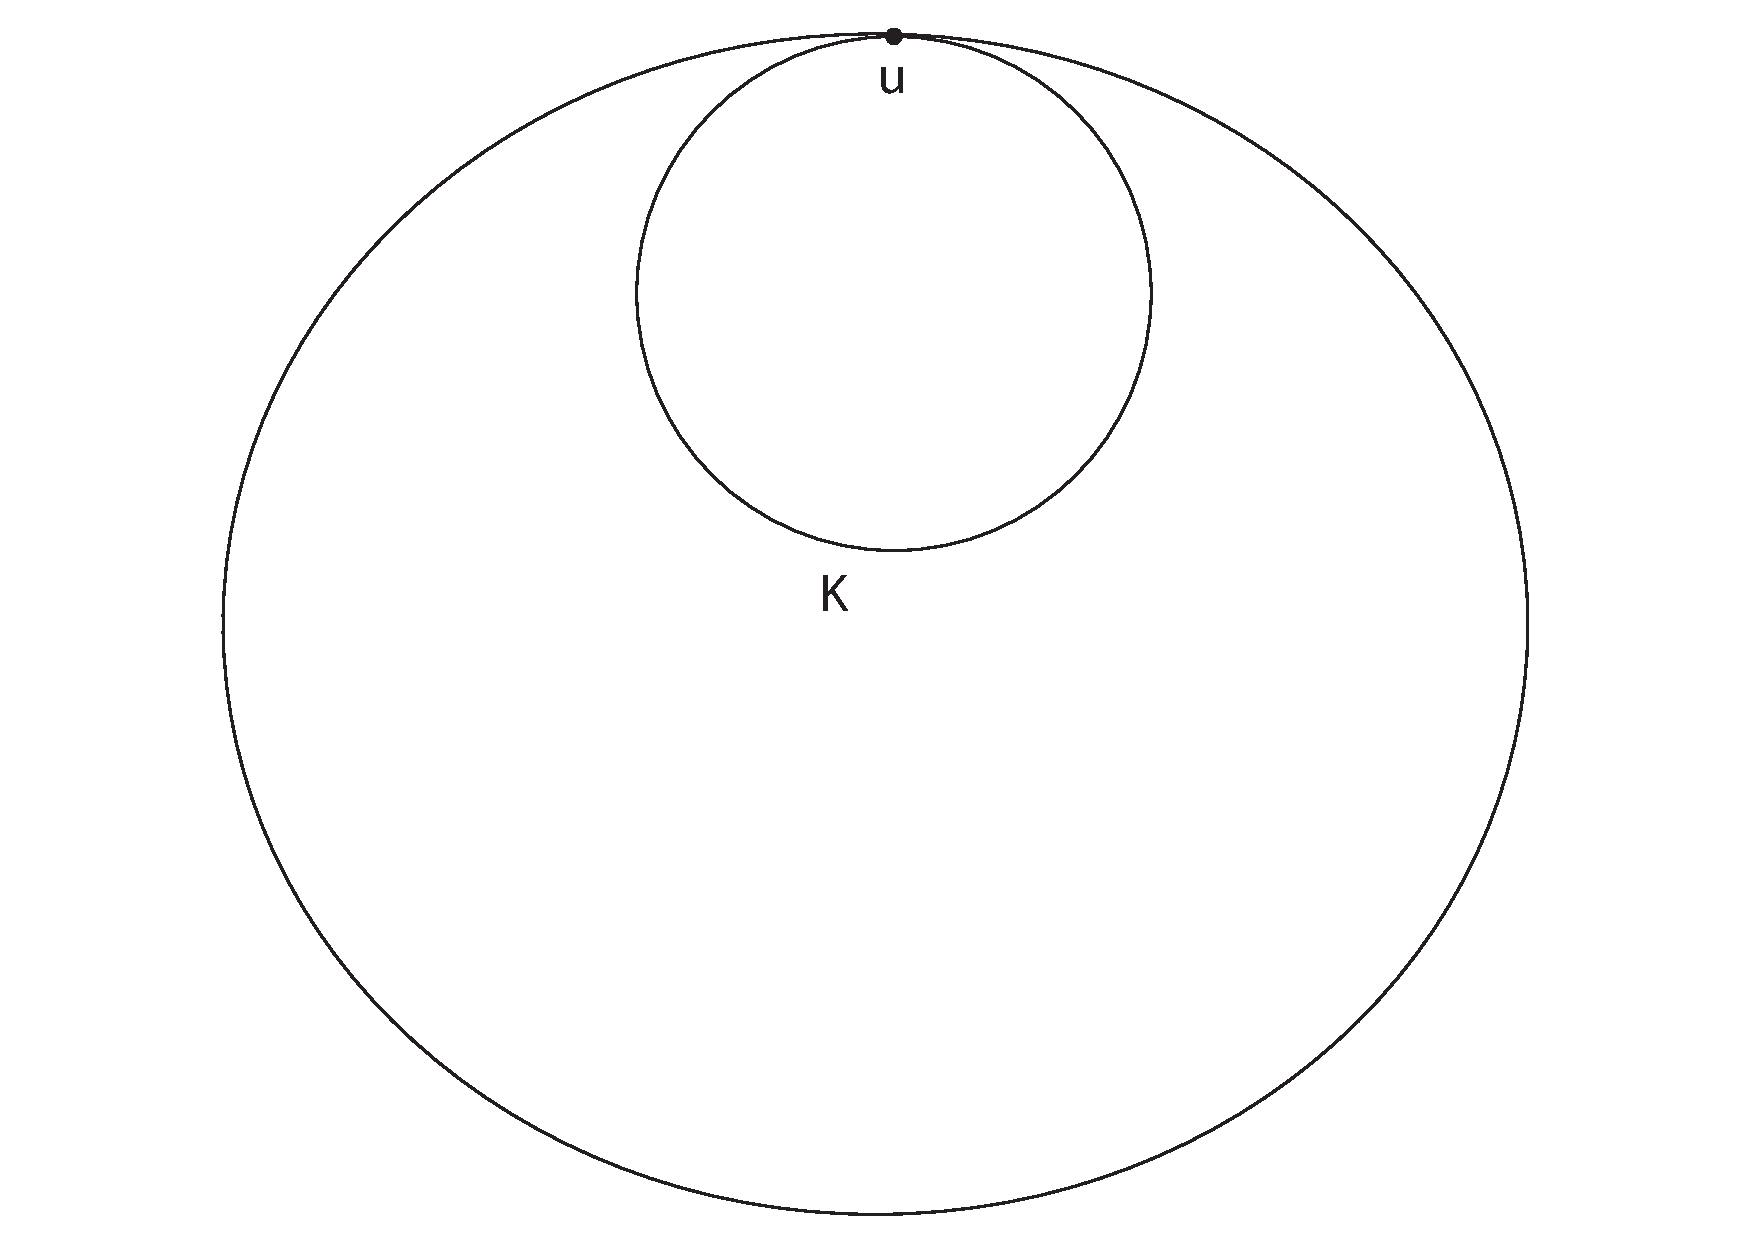
\includegraphics[width=10cm]{lemma5-dibujo1}\\
  \caption{Figura \ref{lemma5-dibujo1}}\label{lemma5-dibujo1}
\end{figure}


Sea $S_{u} < G$ el subgrupo de $G$ que consta de elementos
parab\'olicos con punto en el infinito $u$ y sea $x \in K$, la clase
de equivalencia $S_{u}x$ es un subconjunto de $K$ y podemos
distinguir dos casos.

\begin{enumerate}
\item Los puntos forman una sucesi\'on de puntos equidistantes
cuando $S_{u}$ es dinscontinuo.

\item El conjunto de puntos es denso en todo $K$ cuando $S_{u}$ no
es discontinuo.
\end{enumerate}

Para probar (1), sea $d=min \lbrace d_{H}(x,fx) | f \in S_{u}
\rbrace$ este minimo existe por que si no es asi se tendria un punto
de acumulaci\'on lo cual por hip\'otesis no es posible. Si $y \in
S_{u}x $ es claro que $min \lbrace d_{H}(y,fy) | f \in S_{u} \rbrace
= d$ y de esto concluimos que el conjunto de puntos es equidistante
de distancia $d$. \\

Para el caso (2) por hip\'otesis tenemos que $S_{u}x$ se acumula en
$x$ y queremos ver que se acumula en todo $K$. Sea $k \in K$ un
punto arbitrario y $B_{\epsilon}(k)= \lbrace z \in D| d_{H}(k,z) < \epsilon
\rbrace$ y tomemos $B_{\epsilon}(k) \cap K$, queremos ver que esxiste $x
\in S_{u}x$ tal que $d_{H}(k,x) < \epsilon$ , si dicha $x$ no existe
entonces los desplazamientos  en $K$ de los elementos de $S_{u}$
estarian acotados inferiormente por $\epsilon$ lo cual implicar\'ia que
$S_{u}$ es discontinuo lo que contradice la hip\'otesis, por lo
tanto $S_{u}$ en denso en todo $K$. \\

Ahora supongamos que estamos en el caso (1) y sea $g_{0}$ el
elemento con el menos desplazamiento respecto de $K$
(Fig. \ref{lemma5-dibujo2}) y $f$ un elemento
hiperb\'olico en $G$ tal que su eje $A_{f}$ tiene a $u$ como punto
fijo y cuyo sentido es tal que se aleja de $u$, entonces $fg_{0}f^{-1}$
fija $u$ y es un elemento parab\'olico y por tanto $fg_{0}f^{-1} \in
S_{u}$. \\

\begin{figure}[h]
  \centering
  % Requires \usepackage{graphicx}
  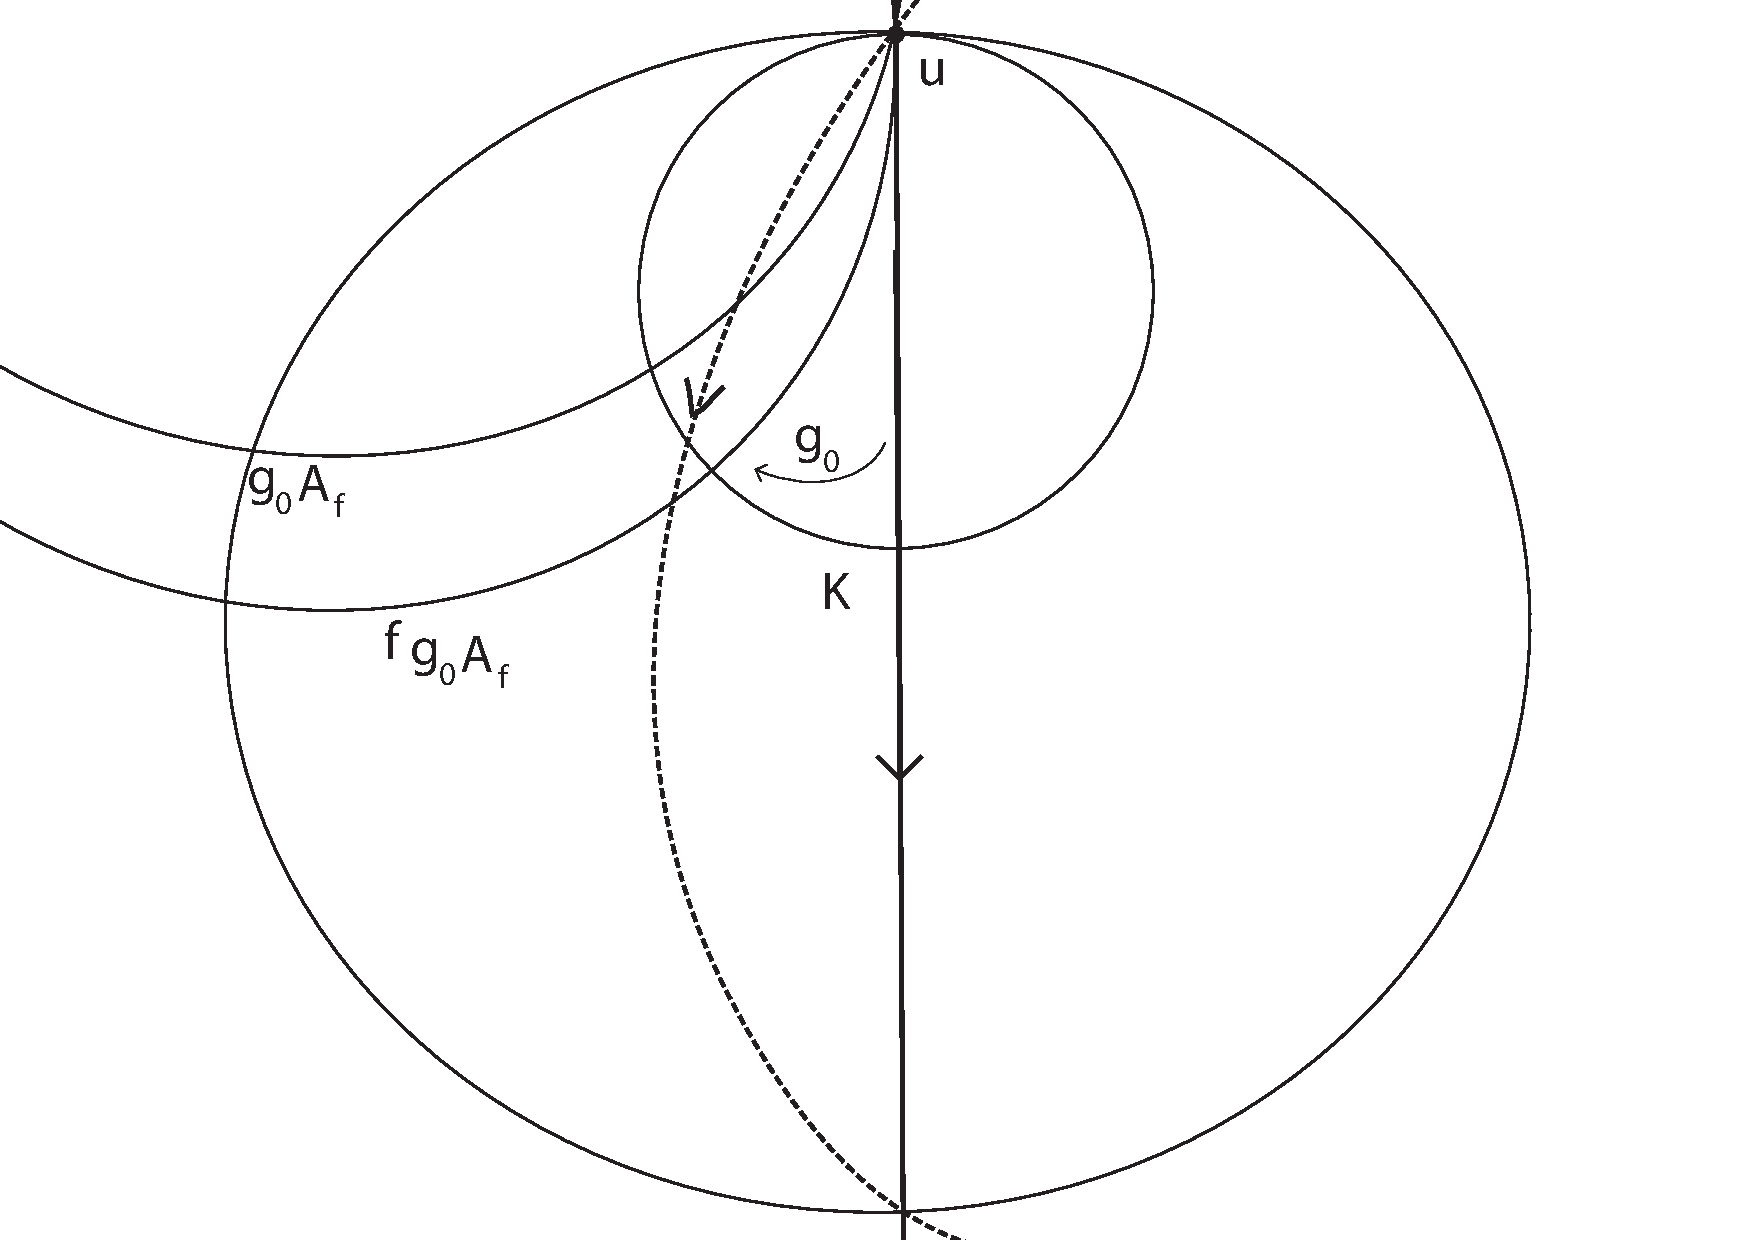
\includegraphics[width=10cm]{lemma5-dibujo2}\\
  \caption{Hiperciclo punteado }\label{lemma5-dibujo2}
\end{figure}

La imagen de $A_{f}$ bajo $fg_{0}f^{-1}$ es claramente la misma que
la de su imagen bajo $fg_{0}$, la recta $fg_{0}A^{f}$ se encuentra
entre $A_{f}$ y $g_{0}A_{f}$, luego el desplazamiento de $fg_{0}f^{-1}$
es menor que el de $g_{0}$ lo cual es una contradicci\'on, por lo
tanto $S_{u}x$ es denso en $K$, es decir los desplazamientos de los
elementos de $S_{u}$ son tan pequeños como se quiera. \\


Como $G$ no tiene a $u$ como punto invariante, sea $g \in G$ tal que
$gu \neq u$. Sean $f_{1},f_{2}$ elementos hiperb\'olicos
pertenecientes a los dos ejes del lema, al menos uno de los
elementos hiperb\'olicos $gf_{j}g^{-1}$ no fija $u$, ya
que $g$ solo puede mover $u$ a los m\'as a uno de los puntos
extremos de $A_{f_{j}}$. Entonces existe en $G$ un elemento
hiperb\'olico $f$ que no deja $u$ invariante. Elijamos ahora un
horociclo $K$ tal que intersecte $A_{f}$ (fig \ref{lemma5-dibujo3}) y elegimos $h$ tal que su
desplazamiento respecto a $K$ ayude a que los ejes $A_{f}$ y
$A_{hf}$ de $f$ y $f'=hfh^{-1}$ respectivamente se intersecten en un
\'angulo arbitrariamente pequeño, en particular elegimos $h$ tal
que
$$sen\phi senh^{2} \frac{1}{2} \lambda_{f} < 1$$

\begin{figure}[h]
  \centering
  % Requires \usepackage{graphicx}
  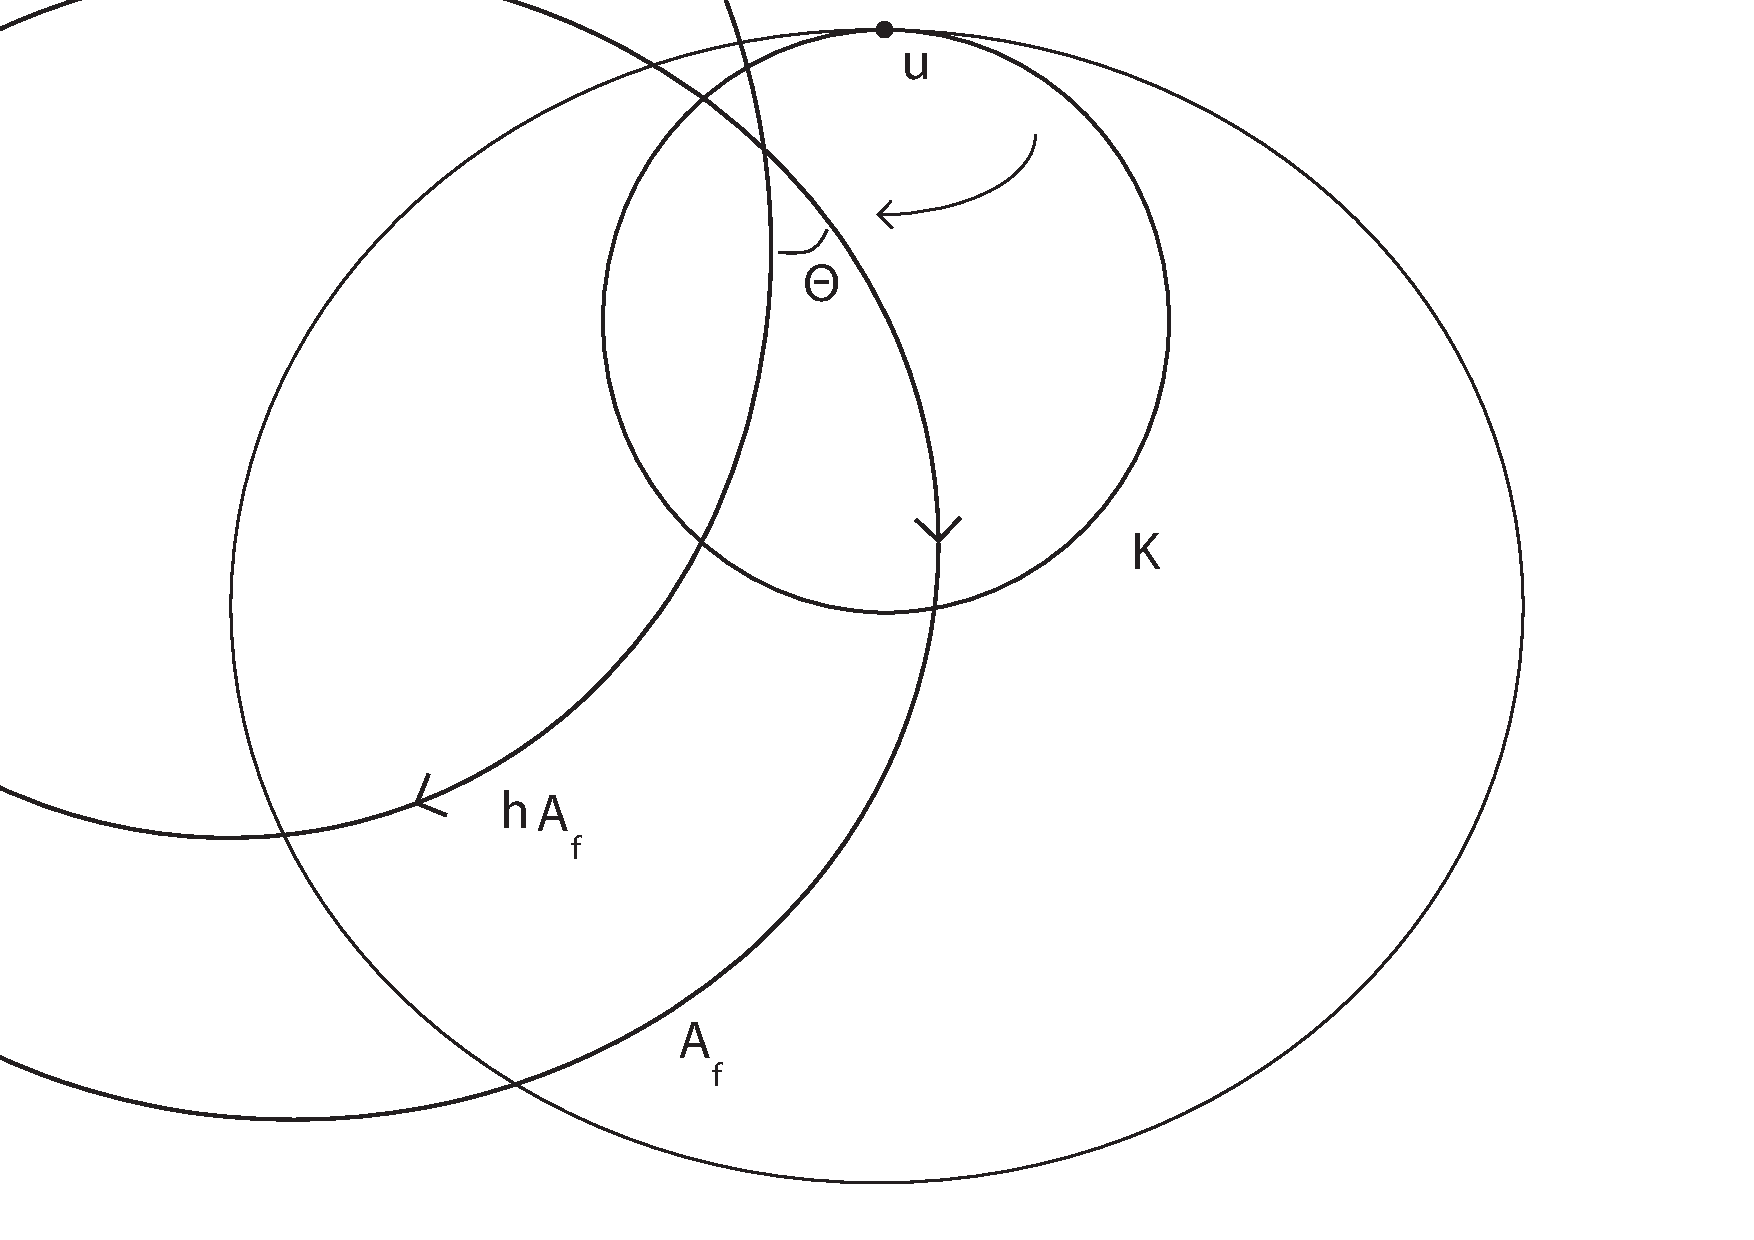
\includegraphics[width=10cm]{lemma5-dibujo3}\\
  \caption{Figura \ref{lemma5-dibujo3}}\label{lemma5-dibujo3}
\end{figure}


Ya que $senh^{2} \frac{1}{2}\lambda_{f}$ es fijo y $sen\phi
\rightarrow 0$ cuando $\phi \rightarrow 0$, y del \textbf{lema} \ref{lema2} se
sigue que $[f,f']$ es el\'iptico. $_{\square}$ \\ \\


\section{El teorema de Nielsen}

Probamos ahora la parte restante del teorema de Nielsen.

Sea $G < PSL(2,\mathbb{R})$ sin puntos invariantes y sin
elementos el\'ipticos. \\

Antes que nada veamos que $G$ no es abeliano. Si los ejes son
divergentes y  $fg = gf$ entonces $fgf^{-1} = g$, pero no es posible
ya que $fgf^{-1}$ fija $fx,fy$ con $x,y $ puntos fijos de $g$, pero
esto implica $fx=y$ y $fy=x$ pero esto implica $f^{2}x=x$, pero
$f^{2}$ fija los mimos puntos que $f$ por tanto no puede fijar los
puntos de $g$. \\

Es an\'alogo si los ejes son paralelos ya que $f$ no puede
intercambiar $x$ y $y$ al mismo tiempo. \\


\begin{figure}[h]
  \centering
  % Requires \usepackage{graphicx}
  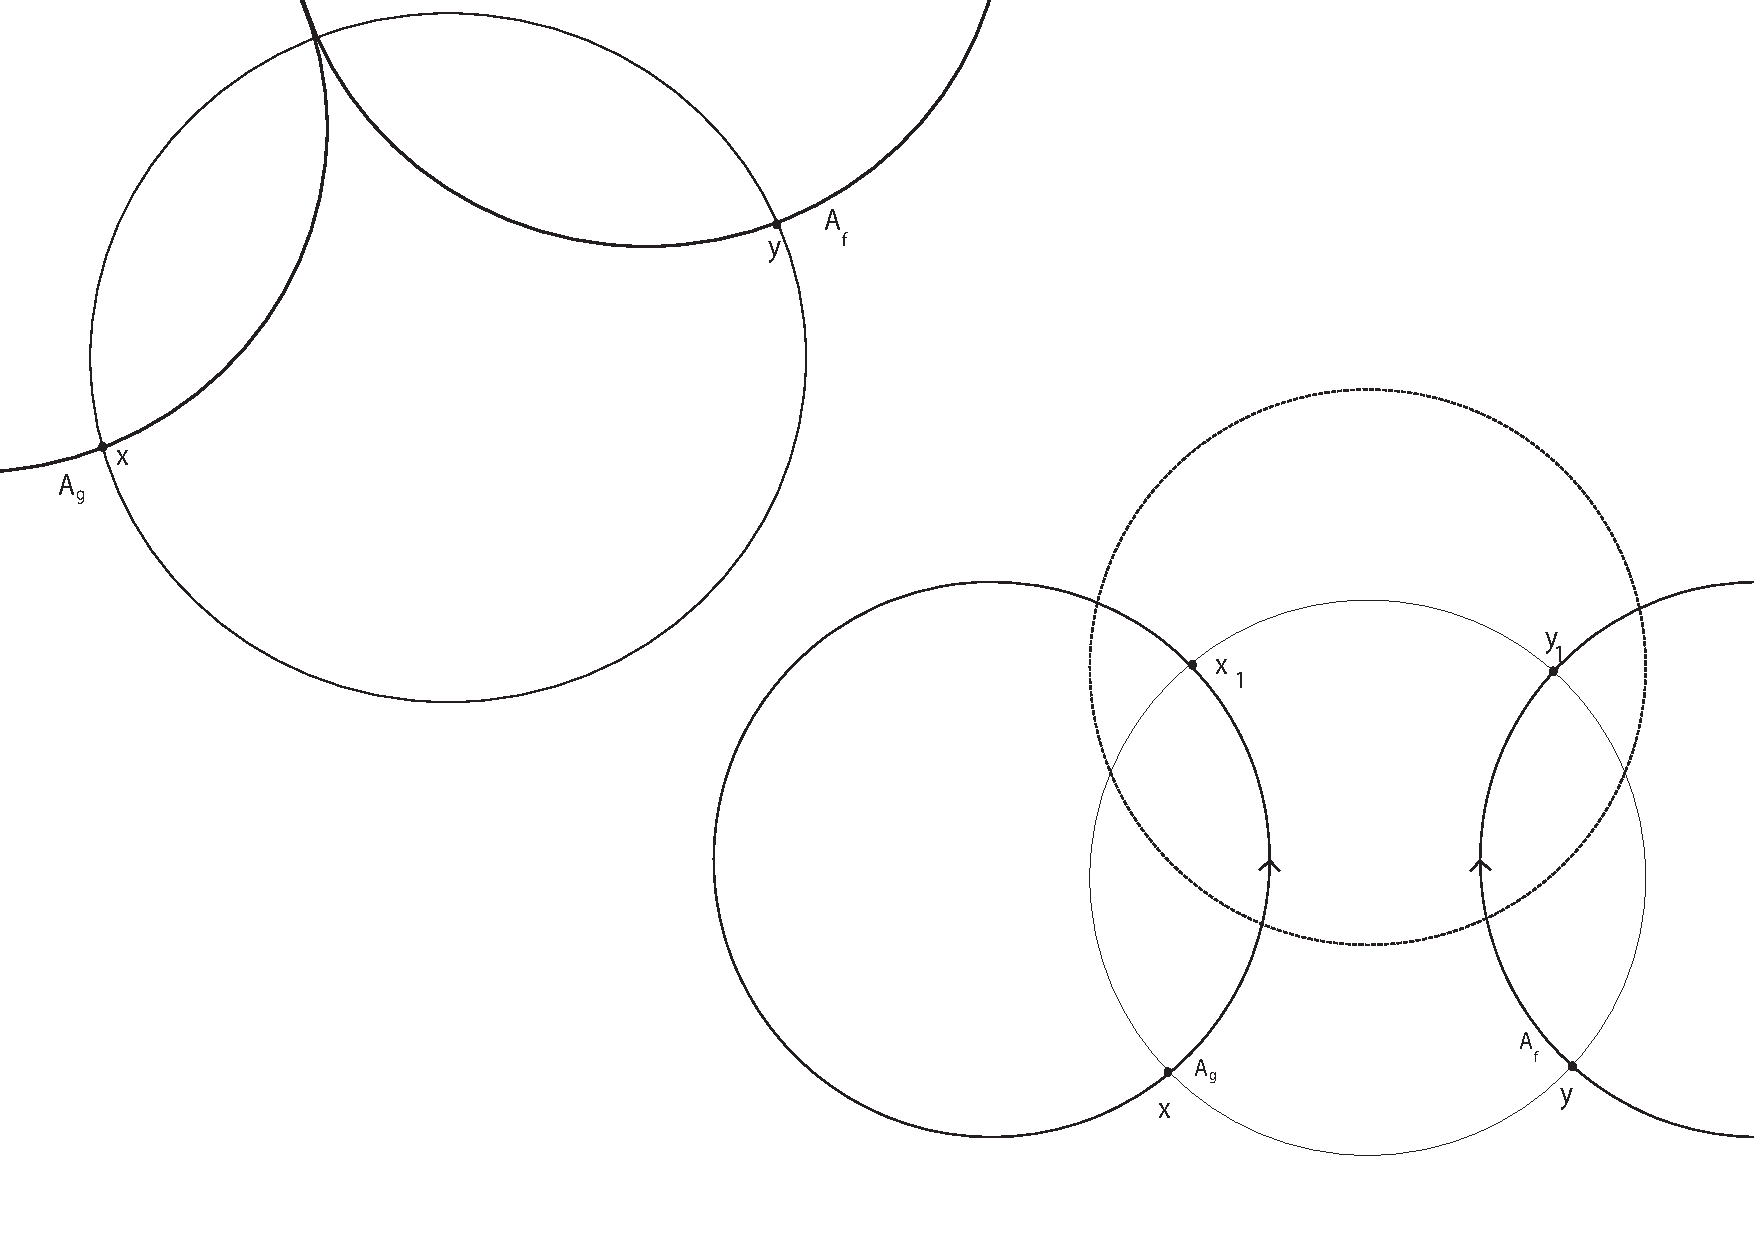
\includegraphics[width=10cm]{lemma6-dibujo-1-2}\\
  \caption{Ejes de f y g paralelos y divergentes}\label{lemma6-dibujo-1-2}
\end{figure}



M\'as a\'un debe haber elementos hiperb\'olicos en $G$, de otro modo
solo tendr\'ia elementos parab\'olicos que por hip\'otesis no
tendrian un punto fijo en com\'un y el lema \ref{lema3} implicar\'ia
una contradicci\'on en este caso. \\

Sea $f$ hiperb\'olico en $G$ y $A_{f} $ su eje y $\lambda_{f}$ la
medida de su desplazamiento, sea $g \in G$ tal que $fg \neq gf$,
entonces $f' = gf^{\pm 1}g^{-1}$ es una hiperb\'olico con el mismo
desplazamiento que $f$ y con eje $gA_{f} \neq A_{f}$ (Por no ser
permutables)(Si $A_{f}=gA_{f} \Rightarrow gfg^{-1}=f$ o
$gfg^{-1}=f^{-1}$. El primer caso es trivial. El segundo caso basta tomar un punto fijo $x$ de $f$ tal que  $g(x)$ no es punto fijo de $f$ (ni de $f^{-1}$) y evaluar en ambos lados de la ecuaci\'on para llegar a una contradicci\'on.) \\

$A_{f},A_{f'}$ no pueden ser paralelas por el lema \ref{lema5}, si
son divergente sea $\delta$ la distancia entre ellas y elijamos $f'$
tal que el exponente de $f$ haga $f$ y $f'$ con desplazamientos
opuestos, por las condiciones impuestas en $G$, $ff'$ no es
el\'iptico y del \ref{lema1} obtenemos

\begin{equation} \label{relacionseno1}
 \  senh \frac{1}{2}
\delta senh \frac{1}{2} \lambda_{f} \geqq 1
\end{equation}

Si $A_{f},A_{f'}$ son concurrentes sea $\phi$ su \'angulo de
intersecci\'on, dado que $[f,f']$ no es una rotaci\'on,  del
\ref{lema2} tenemos

\begin{equation} \label{relacionseno2}
 \ sen \phi senh^{2}\frac{1}{2} \lambda_{f} \geqq 1
\end{equation}

Estas desigualdades se aplican a $g$ fijo y $f$ variando.



\begin{figure}[h]
  \centering
  % Requires \usepackage{graphicx}
  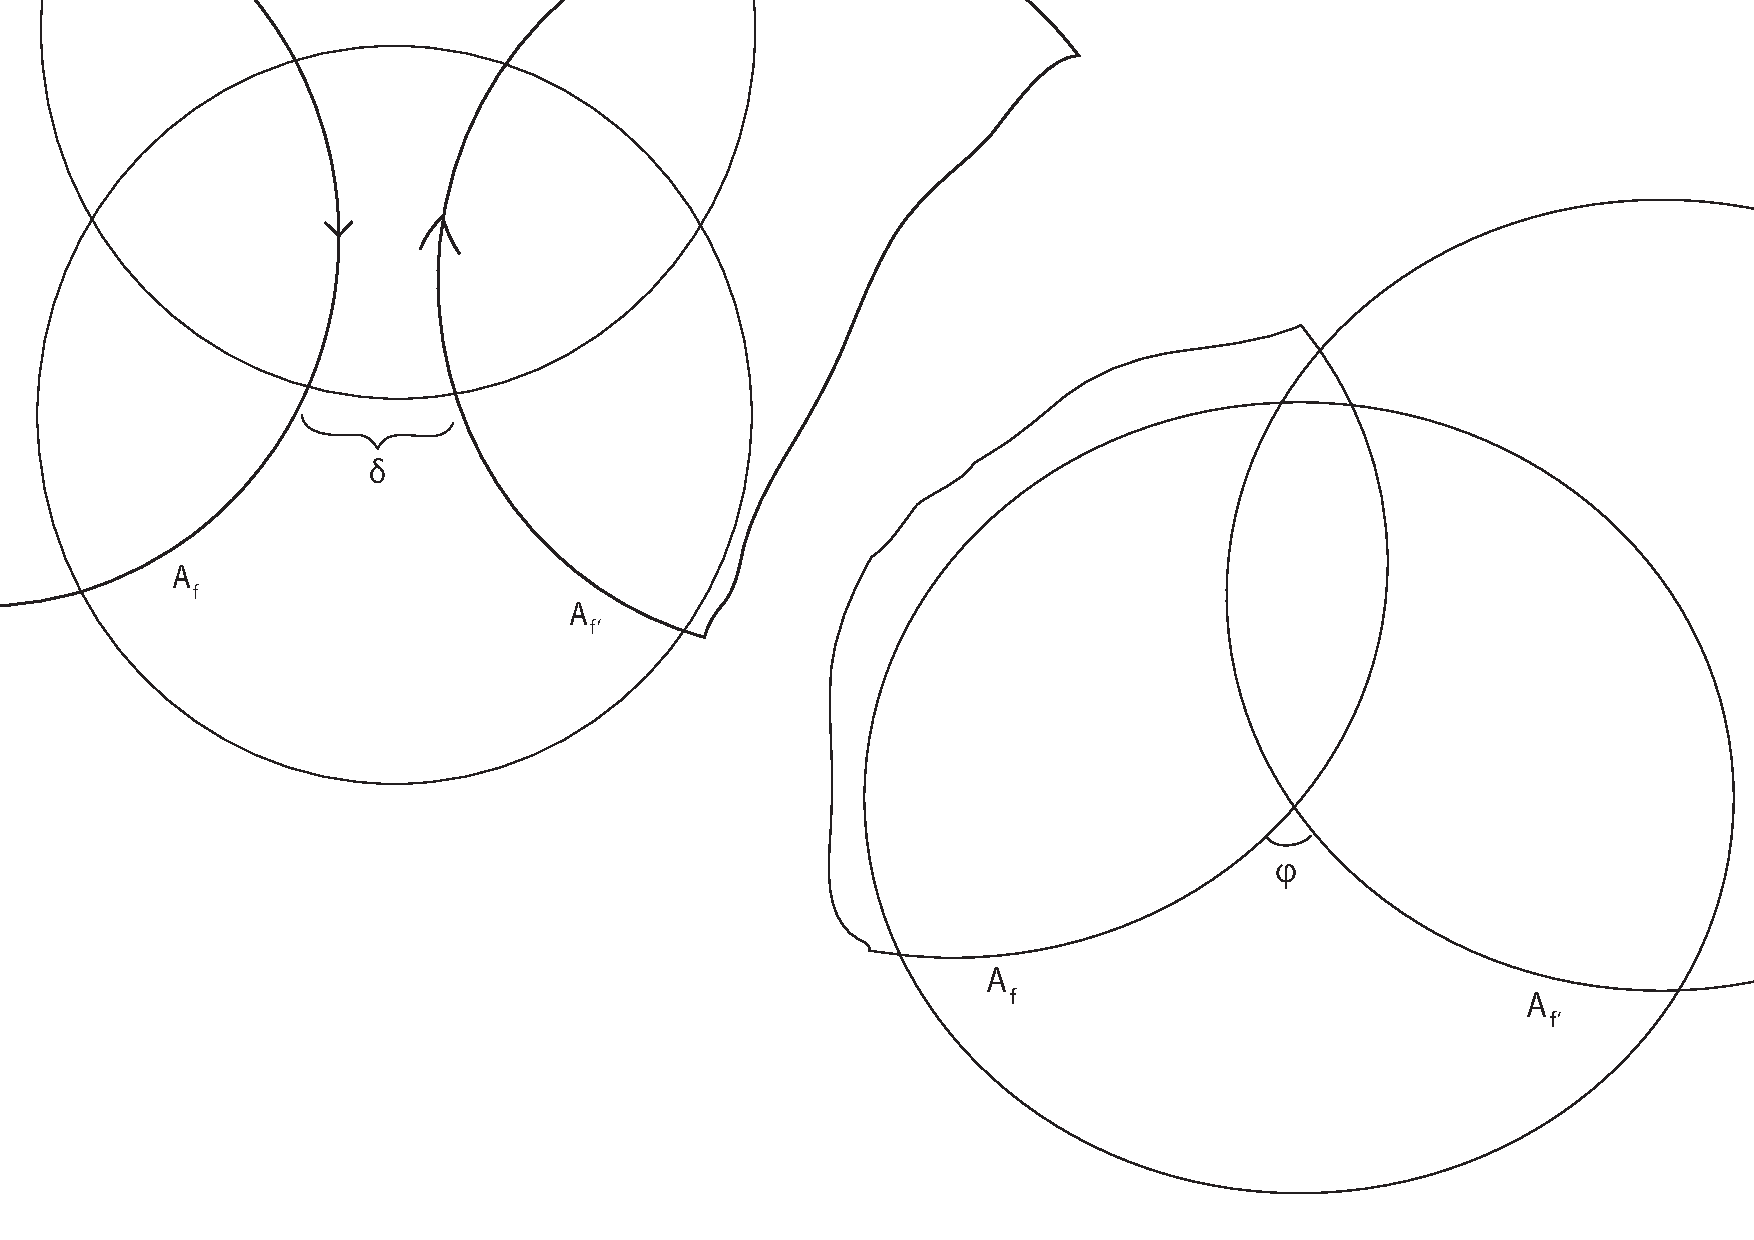
\includegraphics[width=9cm]{lemma6-dibujo-2-4}\\
  \caption{Figura \ref{lemma6-dibujo-2-4}}\label{lemma6-dibujo-2-4}
\end{figure}


Sea $A$ un eje de un elemento hiperb\'olico en $G$, los elementos
hiperb\'olicos que comparten este eje forman un subgrupo abeliano
$S_{A}$ de $G$, sea $g \in G$ un elemento que no tenga como eje a
$A$, es decir que no permuta con los elementos de $S_{A}$, se tiene
que $gA \neq A$. Si $gA$ y $A$ son divergentes digamos que su distancia es $d_{H}(gA,A)= \delta$
si $gA$ y $A$ son concurrentes digamos que se cortan en un \'angulo $\phi$. Dependiendo cual sea el caso aplicaremos \ref{relacionseno1} o \ref{relacionseno2}. \\


Si $f$ varia sobre todos los elementos de $S_{A}$, podemos notar que
todos tienen desplazamiento mayor que un n\'umero positivo distinto
de 1,por las condiciones \ref{relacionseno1} y \ref{relacionseno2} y sabiendo que $senhx \rightarrow 0$ cuando $x \rightarrow 0 $, $\lambda_{f}$ no puede ser arbitrariamente pequeño, m\'as a\'un los desplazamientos no pueden ser arbitrariamente cercanos a la cota, si asi fuera podemos encontrar dos elementos tal que su composici\'on tiene un desplazamiento menor que la cota dada. Entonces $S_{A}$ es discontinuo. Sea $\lambda_{0}$ el desplazamiento mas pequeño de elementos de $S_{A}$ que por lo anterior existe.  \\

Podemos aplicar las mismas desigualdades para $f \in S_{A}$ fijo y
$g $ variando sobre los representantes $g_{1},g_{2},...$ de las
clases de $S_{A} < G$ ($g_{1} \backsim g_{2} \Leftrightarrow
g_{1}S_{A} = g_{2}S_{A} \Leftrightarrow g_{1}g_{2}^{-1} \in S_{A}$).

\begin{rem}
Si $g_{1} \backsim g_{2} \Rightarrow g_{1}A=g_{2}A$ ya que
$g_{1}g_{2}^{-1} = f \in S_{A} \Rightarrow g_{1}g_{2}^{-1}A = fA
\Rightarrow g_{1}g_{2}^{-1}A = A \Rightarrow g_{2}^{-1}A =
g_{1}^{-1}A$
\end{rem}

Los ejes de los elementos hiperb\'olicos $f_{v}=
g_{v}fg_{v}^{-1}$ varian sobre los diferentes ejes de la clase de
equivalencia $GA$ de $A$. \\

Dado que $f_{v}$ tiene el mismo desplazamiento $\lambda_{f}$ que $f$
para todo \'indice $v$, de \ref{relacionseno1} y \ref{relacionseno2} obtenemos que
$senh\frac{1}{2} \delta $ y $sen \phi$ tienen una cota inferior por
lo que $\delta$ y $\phi$ tambi\'en la tienen seg\'un sean
divergentes o concurrentes los ejes $g_{v}A$, esto implica que los
ejes no se acumulan en $D$.  \\


Sea $x \in A$. Todo punto en $Gx$ esta en alg\'un elemento del
conjunto $g_{v}A$. Para un eje dado los puntos $Gx$ que se
encuentran en este eje forman una sucesi\'on de puntos equidistantes
a distancia $\lambda$ (Los puntos en $Gx \cap g_{v}A$ son los puntos
$gx,hx$ tal que $g \backsim h $, luego para $gx,hx \in g_{v}A
\Rightarrow d_{H}(gx,hx)=d_{H}(x,g^{-1}hx), g^{-1}h \in S_{A}
\Rightarrow \lambda_{g^{-1}h} \geqq \lambda_{0}$ (Fig. \ref{lemma6-dibujo6}). \\

\begin{figure}[h]
  \centering
  % Requires \usepackage{graphicx}
  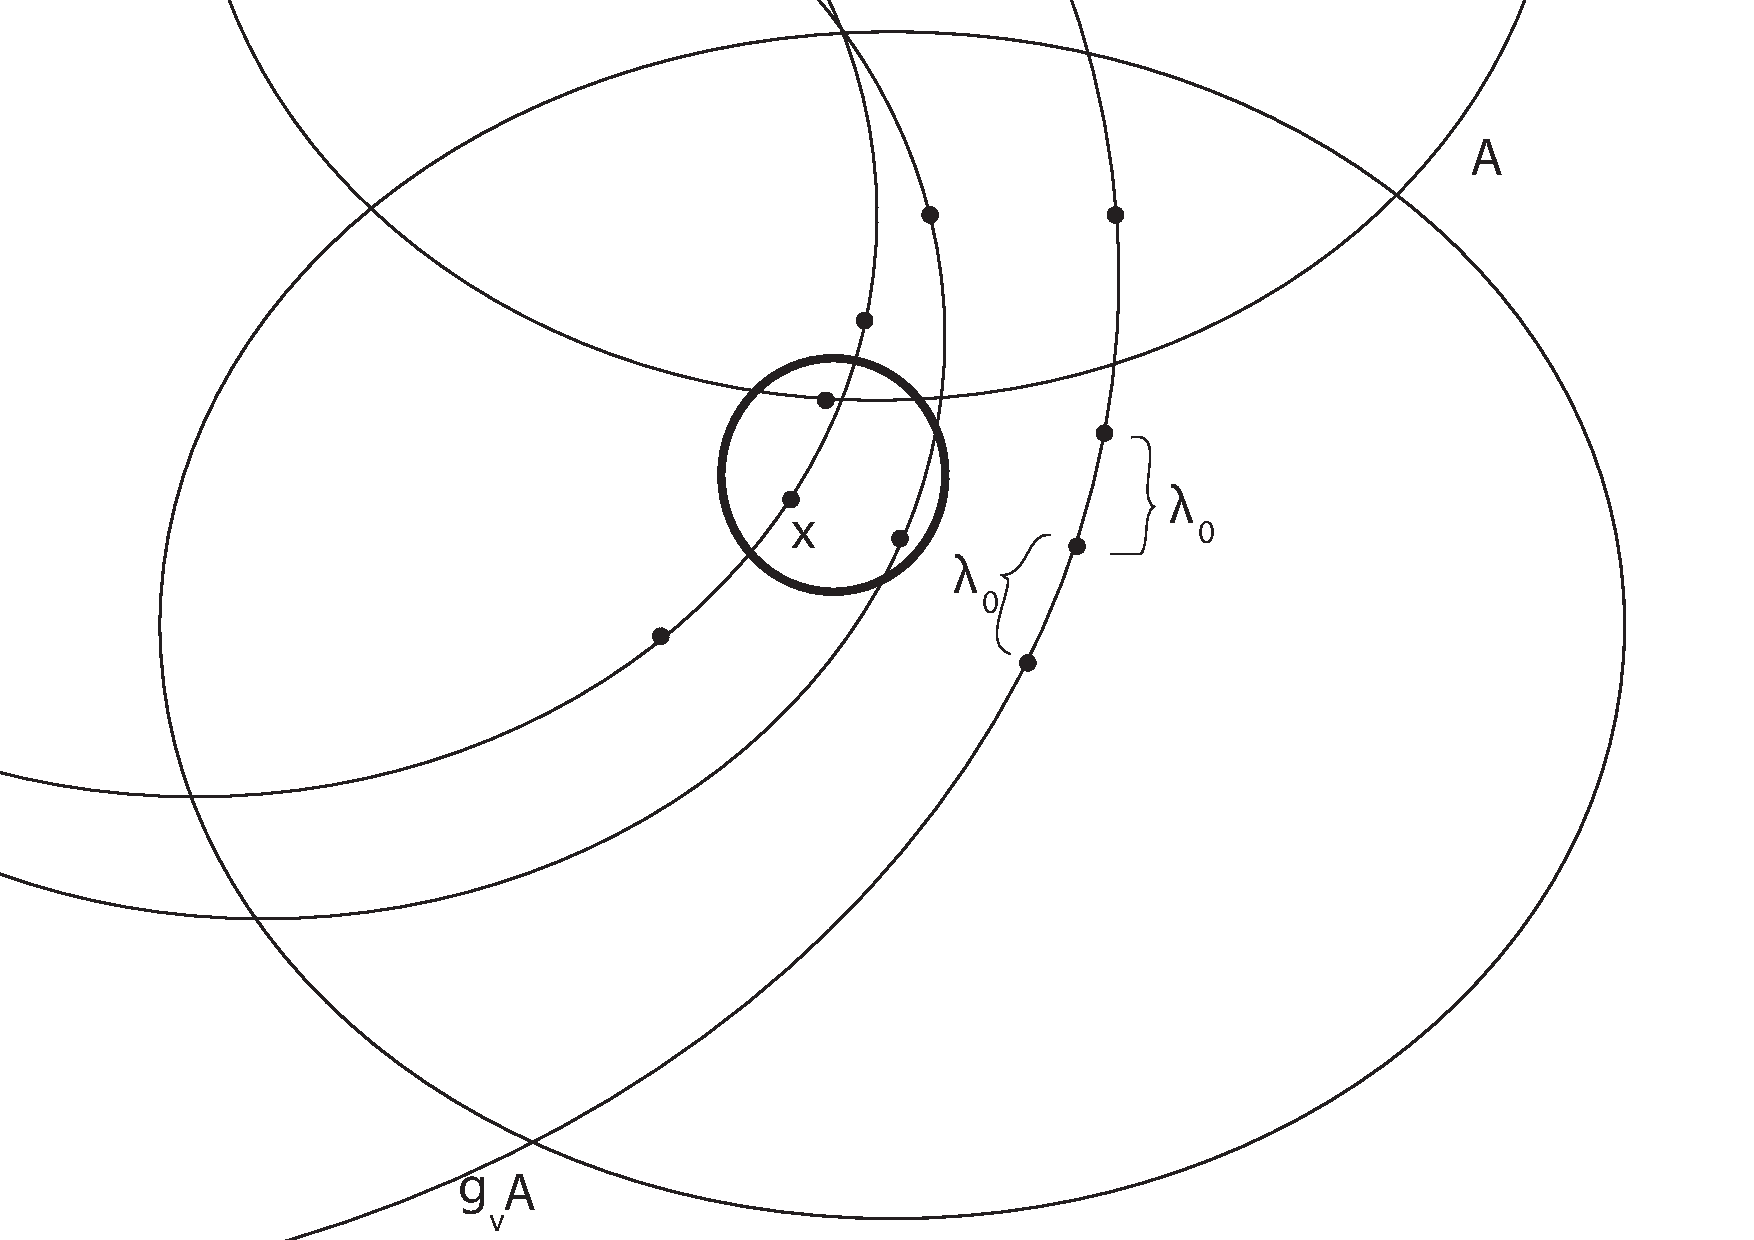
\includegraphics[width=10cm]{lemma6-dibujo6}\\
  \caption{Figura \ref{lemma6-dibujo6}}\label{lemma6-dibujo6}
\end{figure}


El c\'irculo con centro $x$ y radio $\frac{1}{2} \lambda_{0}$
no puede contener mas de un punto de dicha sucesi\'on en su
interior, entonces el n\'umero de puntos en $Gx$ dentro de este
c\'irculo es a lo m'as igual al n\'umero de ejes $g_{v}A$ que cortan
al c\'irculo, este n\'umero es finito ya que los ejes $g_{v}A$ no se
acumulan en $D \  \therefore \ x$ no es punto de acumulaci\'on de
$Gx$. $_{\square}$



\section{Un ejemplo de un grupo discreto}

En el cap\'itulo \ref{cha:grupo schottky} hallamos un grupo de Schottky que es un subgrupo discreto de isometrias hiperb\'olicas, m\'as a\'un sabemos que todos los elementos no triviales del grupo de Schottky son loxodr\'omicos, en nuestro caso hiperb\'olicos, excepto por la identidad, para que podamos validar el teorema de Nielsen en este grupo debemos verificar que se cumplen las condiciones del teorema. Los generadores del grupo de Schottky son hiperb\'olicos por lo cual cada uno tiene una geodesica invariante, podemos usar las matrices del grupo de monodrom\'ia de la ecuaci\'on diferencial hipergeometrica \ref{Matrices_teorema_monodromia_grupo} que son conjugadas a los generadores del grupo de Schottky;

$$  A_{0} =  \begin{pmatrix}
 1& 0\\
 0& \varepsilon (-c)
 \end{pmatrix}  ,\ \ \
A_{1} = P ^{-1}\begin{pmatrix}
 1& 0\\
 0& \varepsilon (c-a-b)
 \end{pmatrix} P
$$


Notamos que $A_{0}$ fija $0,\infty$ y por tanto deja invariante la geod\'esica que los une, podemos ver que $A_{1}$ fija $P^{-1}(0)$ y $P^{-1}(\infty)$ y dado que conocemos $P^{-1}$ podemos calcular ambos valores, por un lado $P^{-1}(0)= \frac{-C}{D}$ por otro lado $P^{-1}(\infty) = \frac{-A}{B}$, y por tanto deja invariante la geod\'esica que une estos dos puntos. Mas abajo probamos que estos dos ejes necesariamente son divergentes.

 En nuestro caso tenemos un grupo de Schottky con dos generadores, sabemos que es libre y tambi\'en es no elemental (\ref{def:elemental}). En \cite{Beardon} encontramos un teorema que dice que para un grupo de transformaciones hiperb\'olicas con las caracteristicas anteriores ser discreto equivale a que act\'ue de manera discontinua seg\'un \ref{def:discontinuo1}, de igual manera en \cite{Beardon} encontramos que \ref{def:discontinuo1} implica \ref{def:discontinuo2}.

 Por otro lado $\Lambda_{\theta}$ posee, salvo la identidad, solo elementos hiperb\'olicos, para aplicar el teorema de Nielsen necesitamos adem\'as que el grupo no tenga ni puntos fijos ni rectas invariantes como mencionamos arriba. En \cite{Beardon} encontramos el siguiente teorema;

\begin{thm}
 Dos transformaciones de Mobius $g,h$ tienen un punto fijo en $\widehat{\mathbb{C}}$ si y solo si $tr[g,h]=2$
\end{thm}

 Haciendo los calculos correspondientes a las matrices asociadas a $\gamma_{1},\gamma_{2}$ obtenemos que; $tr[\gamma_{1},\gamma_{2}] = \frac{2T^{2}(R^{2}-C^{2}) + C^{2}(T^{4} +1)}{T^{2}R^{2}}$, si suponemos que $tr[\gamma_{1},\gamma_{2}]=2$ obtenemos que $C^{2}=0$ o que $T= \pm 1$, ninguno de estos casos es posible debido a las condiciones exigidas, por lo que $tr[\gamma_{1},\gamma_{2}] \neq 2$ es decir $\gamma_{1},\gamma_{2}$  no tienen puntos fijos en $\widehat{\mathbb{C}}$ (en particular no los tiene en $D$) y dado que tienen ejes diferentes, estos necesariamente son divergentes de otro modo su intersecci\'on ser\'ia un punto fijo, por tal motivo no hay rectas invariantes en el grupo generado por estos elementos.Aplicando el teorema de Nielsen se puede concluir que $\Lambda_{\theta}$ es discontinuo en $D$.

Todo lo anterior nos permite afirmar que la familia de  grupos de Schottky hallada en \ref{cha:grupo schottky} son ejemplos en donde podemos verificar el teorema de Nielsen. En la actualidad existen muchos resultados que nos dan la misma informaci\'on que este teorema pero la exposici\'on geom\'etrica de este resultado sigue siendo admirable gracias a su demostraci\'on basada en su mayoria en la geometr\'ia hiperb\'olica pura.


%----------------------------------------------------------------------

